%%%%%%%%%%%%%%%%%%%%%%%%%%%%%%%%%%%%%%%%%
% Maggi Memoir Thesis (WriteLaTeX Version - Compiles with pdflatex)
% XeLaTeX Template
% Version 1.0 (22/12/13)
%
% This template has been downloaded from:
% http://www.LaTeXTemplates.com
%
% Original authors:
% Federico Maggi (fede@maggi.cc) with extensive modifications by:
% Vel (vel@latextemplates.com)
%
% License:
% CC BY-NC-SA 3.0 (http://creativecommons.org/licenses/by-nc-sa/3.0/)
%
% Important note:
% Most of the document content and packages are specified within structure.tex
% so if you need to make modifications to the template have a look there first!
%
%%%%%%%%%%%%%%%%%%%%%%%%%%%%%%%%%%%%%%%%%

%----------------------------------------------------------------------------------------
%	PACKAGES AND OTHER DOCUMENT CONFIGURATIONS
%----------------------------------------------------------------------------------------

\documentclass[10pt,a4paper,twoside]{memoir} % Change font size here (allowable values are 9pt-12pt), change the paper size, specify one or two sided printing and specify whether to show trimming lines

%----------------------------------------------------------------------------------------
%	VARIOUS REQUIRED PACKAGES AND CONFIGURATIONS
%----------------------------------------------------------------------------------------

\usepackage[T1]{fontenc} % Support for more character glyphs
\usepackage[round]{natbib}\citeindextrue % Round brackets around citations, change to square for square brackets
\usepackage{graphicx} % Required to include images
\usepackage{color} % Required for custom colors
\usepackage{amsmath,amssymb,theorem} % Math packages
\usepackage{listings} % Required for including snippets of code
\usepackage{booktabs} % Required for better horizontal rules in tables
\usepackage{xspace} % Provides the ability to use an intelligent space which is used in \institution and \department
\usepackage[printonlyused,withpage]{acronym} % Include a list of acronyms
\usepackage{rotating} % Allows tables and figures to be rotated
\usepackage{hyperref} % Required for links and changing link options
\usepackage{microtype} % Slightly tweak font spacing for aesthetics
\usepackage[en-GB]{datetime2}
\usepackage[linesnumbered,ruled,vlined]{algorithm2e}

\hypersetup{colorlinks, breaklinks, linkcolor=black,citecolor=black,filecolor=black,urlcolor=black} % Set up hyperlinks including colors for references, urls and citations

%\definecolor{c64}{rgb}{.063,0,.612} % Example color definition, the color can be used with the \color{name} command

\makeatletter
\renewcommand{\fnum@figure}{\textsc{\figurename~\thefigure}} % Make the "Figure 1.1" text in small caps
\makeatother

%----------------------------------------------------------------------------------------
%	PAGE LAYOUT
%----------------------------------------------------------------------------------------

% The memoir class used in this template contains the ability to set the stock paper size and the trimmed size independently. It also has the ability to show trim lines showing where stock paper should be trimmed to get the final book size. This can all be a bit confusing so please see the memoir class documentation for more information.

% By default, the paper size is a4paper which is 29.7cm × 21cm. To change this, simply change "a4paper" in the \documentclass[a4paper,...]{memoir} command in thesis.tex to another size such as "letterpaper".
% By default, the trimmed size is 24cm x 17cm and trim lines are shown. To remove trim lines, simply remove "showtrims" from the \documentclass[showtrims,...]{memoir} command in thesis.tex. The size of the trimmed content is set with the \settrimmedsize{}{} command below.
% If you wish to remove trims and set the content to fit the paper size (i.e. no trimming at all), all you have to do is remove "showtrims" as above and comment out the \settrimmedsize{}{} command below.

%\setstocksize{24cm}{17cm} % Uncomment to manually set the stock size and override the setting in \documentclass
%\settrimmedsize{24cm}{17cm}{*} % Change the trimmed area size or comment out this line entirely to fit the content to the paper size without trimming
\setlrmarginsandblock{37.125mm}{*}{0.9} % The first bracket specifies the spine margin, the second the edge margin and the third the ratio of the spine to the edge. Only one or two values are required and the remaining one(s) can be a star (*) to specify it is not needed. By default the edge margin is 10% smaller and
\setulmarginsandblock{37.125mm}{*}{*} % The first bracket specifies the upper margin, the second the lower margin and the third the ratio of the upper to the lower. Only one or two values are required and the remaining one(s) can be a star (*) to specify it is not needed.
\setmarginnotes{17pt}{51pt}{\onelineskip} % The size of marginal notes, the three values in curly brackets are \marginparsep, \marginparwidth and \marginparpush
\setheadfoot{\onelineskip}{2\onelineskip} % Sets the space available for the header and footer
\setheaderspaces{*}{2\onelineskip}{*} % Sets the spacing above and below the header
\setlength{\trimtop}{0pt} % Sets the spacing above the trimmed area, i.e. moved the trimmed area down the page if positive

% Comment the two lines below to reverse the position of the trimmed content on the stock paper, i.e. odd pages will have content on the right side instead of the left and even pages will have content on the left side instead of the right
\setlength{\trimedge}{\stockwidth}
\addtolength{\trimedge}{-\paperwidth}

\checkandfixthelayout % Makes sure your specifications are correct and implements them in the document

%----------------------------------------------------------------------------------------
%	CHAPTER HEADING STYLE
%----------------------------------------------------------------------------------------

\makeatletter
\makechapterstyle{thesis}{
\renewcommand{\chapternamenum}{}
\setlength{\beforechapskip}{0pt}
\setlength{\midchapskip}{0pt}
\setlength{\afterchapskip}{0pt}
\renewcommand{\chapnamefont}{\HUGE}
\renewcommand{\chapnumfont}{\chapnamefont}
\renewcommand{\chaptitlefont}{\chapnamefont}
\renewcommand{\printchapternum}{}
\renewcommand{\afterchapternum}{}
\renewcommand{\printchaptername}{}
\renewcommand{\afterchaptertitle}{\chapnumfont\hfill\thechapter\\\vspace*{-.3cm}\hrulefill\vspace*{2cm}\\}
}
\makeatother

%----------------------------------------------------------------------------------------
%	TABLE OF CONTENTS DEPTH
%----------------------------------------------------------------------------------------

\maxsecnumdepth{subsubsection}
\maxtocdepth{subsection}

%----------------------------------------------------------------------------------------
%	MATH THEOREM DEFINITIONS
%----------------------------------------------------------------------------------------

\theoremstyle{plain}
\newtheorem{thm}{Theorem}[section] % Defines the theorem environment
\newtheorem{prop}[thm]{Proposition} % Defines the proposition environment
\newtheorem{proof}{Proof}[section] % Defines the proof environment
\newtheorem{definition}{Definition}[section] % Defines the definition environment
\newtheorem{example}{Example}[section] % Defines the example environment
\newtheorem{rem}{Remark} % Defines the remark environment
\newtheorem{note}{Note}[section] % Defines the note environment

%----------------------------------------------------------------------------------------
%	CODE SNIPPET CONFIGURATION
%----------------------------------------------------------------------------------------

\lstset{
  basicstyle=\ttfamily\small,
  basewidth=0.55em,
  showstringspaces=false,
  numbers=left,
  numberstyle=\tiny,
  numbersep=2.5pt,
  keywordstyle=\bfseries\ttfamily,
  breaklines=true
}
% Examples of list environments for different programming languages, you will likely need to specify your own
\lstnewenvironment{pseudoc}{\lstset{frame=lines,language=C,mathescape=true}}{}
\lstnewenvironment{logs}{\lstset{frame=lines,basicstyle=\footnotesize\ttfamily,numbers=none}}{}
\lstnewenvironment{cc}{\lstset{frame=lines,language=C}}{}
\lstnewenvironment{c64}{\lstset{backgroundcolor=\color{c64},basewidth=0.65em,basicstyle=\commodoreface\color{c64light},numbers=none,framerule=10pt,rulecolor=\color{c64light},frame=tb,framexbottommargin=30pt}}{}
\lstnewenvironment{html}{\lstset{frame=lines,language=html,numbers=none}}{}
\lstnewenvironment{pseudo}{\lstset{frame=lines,mathescape=true,morekeywords={learn_string_domain, save_model}}}{}
\lstnewenvironment{pseudoctiny}{\lstset{language=C,mathescape=true,basicstyle=\tiny\sffamily}}{}
\lstnewenvironment{cctiny}{\lstset{language=C,basicstyle=\tiny\sffamily}}{}
\lstnewenvironment{pseudotiny}{\lstset{mathescape=true,basicstyle=\tiny\sffamily}}{} % Include the file containing the code defining the structure and style of the document

%------------------------------------------------
% Thesis Information

\title{Implementation of a 6 DoF EKF-SLAM for Leonardo Drone Contest} % Thesis title

\author{Diego Emanuel Avila} % Author name

\date{December 2020} % The date

\newcommand{\institution}{ {\Large POLITECNICO DI MILANO}\xspace } % University/institution name

\newcommand{\department}{AIR Lab - Artificial Intelligence and Robotics Lab \\ Dipartimento di Elettronica, Informazione e Bioingegneria\xspace} % Department name

%------------------------------------------------
% Fonts

\renewcommand*{\acffont}[1]{{\normalsize\itshape #1}} % Font style for the acronym text (e.g. Do It Yourself)
\renewcommand*{\acfsfont}[1]{{\normalsize\upshape #1}} % Font style for the acronym in bracket (e.g. (DIY))

%------------------------------------------------
% Hyphenations

\hyphenation{} % Specify custom hyphenation points in words with dashes where you would like hyphenation to occur, or alternatively, don't put any dashes in a word to stop hyphenation altogether

%----------------------------------------------------------------------------------------
%	TITLE PAGE
%----------------------------------------------------------------------------------------

\renewcommand{\maketitlehooka}{
\centering
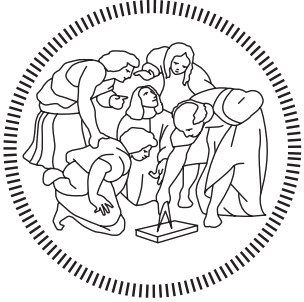
\includegraphics[width=5cm]{Figures/polimi-logo.png}\\[.2cm] % Institution logo
\institution\\[0.3cm] % Print institution name
\emph{\department}\\[.2cm] % Print department name
MSc. in Computer Science and Engineering % Degree or other information
\par
\hrulefill
\vfill}
\renewcommand{\maketitlehookb}{\vfill}
\renewcommand{\maketitlehookc}{
\vfill
\begin{flushleft}
Supervisor:\\
\textbf{Prof. Matteo Matteucci}\\[.3cm]
\end{flushleft}
\vfill}
\preauthor{\begin{flushright}Author:\\\bfseries} % Text prior to the author name - right aligned and bold
\postauthor{ \\ Matricola: 903988\end{flushright}} % After the author name, stop right alignment

%----------------------------------------------------------------------------------------

\makeindex % Write an index file

\begin{document}

\begin{titlingpage}
\maketitle % Print the title page
\end{titlingpage}

\frontmatter % Use roman page numbering style (i, ii, iii, iv...) for the pre-content pages

%----------------------------------------------------------------------------------------
%	PREFACE
%----------------------------------------------------------------------------------------

\section*{Preface}
Some preface

\begin{flushright}
\textsc{\theauthor}\\
Milano\\
\DTMlangsetup{showdayofmonth=false}
\today
\DTMlangsetup{showdayofmonth=true}
\end{flushright}

\cleartoverso % Force a break to an even page

%----------------------------------------------------------------------------------------
%	ABSTRACT
%----------------------------------------------------------------------------------------

\begin{abstract}
Abstract

\end{abstract}

\cleartoverso % Force a break to an even page

%----------------------------------------------------------------------------------------
%	TABLE OF CONTENTS
%----------------------------------------------------------------------------------------

\tableofcontents* % Print the table of contents

\cleartoverso % Force a break to an even page

%----------------------------------------------------------------------------------------
%	LIST OF FIGURES
%----------------------------------------------------------------------------------------

\listoffigures % Print the list of figures

\cleartoverso % Force a break to an even page

%----------------------------------------------------------------------------------------
%	LIST OF TABLES
%----------------------------------------------------------------------------------------

\listoftables % Print the list of tables

\cleartoverso % Force a break to an even page

%----------------------------------------------------------------------------------------
%	ACRONYMS
%----------------------------------------------------------------------------------------

\chapter{List of Acronyms}
\begin{acronym}\addtolength{\itemsep}{-\baselineskip}
  \acro{IDL}{Interface Description Language}
  \acro{ROS}{Robot Operating System}
  \acro{RViz}{ROS Visualization}
  \acro{SLAM}{Simultaneous Localization And Mapping}
  \acro{EKF}{Extended Kalman Filter}
  \acro{KF}{Kalman Filter}
  \acro{NEES}{Normalized Estimation Error Squared}
  \acro{ENU}{East-North-Up}
  \acro{NED}{North-East-Down}
  \acro{RTAB-Map}{Real-Time Appearance-Based Mapping}
\end{acronym} % Include a List of Acronyms section using acronyms.tex where they are defined

\cleartoverso % Force a break to an even page

%----------------------------------------------------------------------------------------
%	COLOPHON
%----------------------------------------------------------------------------------------

\thispagestyle{empty} % Remove all headers and footers from this page

%\vspace*{2em}
%\renewcommand{\abstractname}{Colophon}
%\begin{abstract}
%This document was typeset using the \textsf{XeTeX} typesetting system created by the Non-Roman Script Initiative and the memoir class created by Peter Wilson. The body text is set 10pt with~Adobe Caslon Pro. Other fonts include \texttt{Envy Code R}, \textsf{Optima Regular} and. Most of the drawings are typeset using the \textsf{TikZ/PGF} packages by Till Tantau.
%\end{abstract}
%\vfill

%----------------------------------------------------------------------------------------
%	CONTENT CHAPTERS
%----------------------------------------------------------------------------------------

\mainmatter % Begin numeric (1,2,3...) page numbering

\chapterstyle{thesis} % Change the style of the Chapter header to that defined in structure.tex

\pagestyle{Ruled} % Include the chapter/section in the header along with a horizontal rule underneath

\chapter{Introduction}
\label{introduction}

Network connected devices such as personal computers, mobile phones, or gaming consoles are nowadays enjoying immense popularity. In parallel, the Web and the humongous amount of services it offers have certainly became the most ubiquitous tools of all the times. \textsf{Facebook} counts more than 250 millions active users of which 65 millions are using it on mobile devices; not to mention that more than 1 billion photos are uploaded to the site \emph{each   month}~\citep{facebook-stats}. And this is just one, popular website. One year ago, \textsf{Google} estimated that the approximate number of unique \acp{URL}\index{URL} is 1 trillion~\citep{google-is-big}, while \texttt{YouTube} has stocked more than 70 million videos as of March 2008, with 112,486,327 views just on the most popular video as of January 2009~\citep{social-media-stats}. And people from all over the world inundate the Web with more than 3 million tweets \emph{per day}. Not only the Web 2.0 has became predominant; in fact, thinking that on December 1990 the Internet was made of \emph{one} site and today it counts more than 100 million sites is just astonishing~\citep{internet-timeline}.

The Internet and the Web are huge~\citep{inetworldstats}. The relevant fact, however, is that they both became the most advanced workplace. Almost every industry connected its own network to the Internet and relies on these infrastructures for a vast majority of transactions; most of the time monetary transactions. As an example, every year \textsf{Google} looses approximately 110 millions of US Dollars in ignored ads because of the \emph{``I'm feeling lucky''} button. The scary part is that, during their daily work activities, people typically pay poor or no attention at all to the risks that derive from exchanging any kind of information over such a complex, interconnected infrastructure. This is demonstrated by the effectiveness of social engineering~\citep{deception} scams carried over the Internet or the phone~\citep{social-engineering-fundamentals}. Recall that 76\% of the phishing is related to finance. Now, compare this landscape to what the most famous security quote states.

\begin{quotation}
  ``The only truly secure computer is one buried in concrete, with the   power turned off and the network cable cut''.
   ---\emph{Anonymous}
\end{quotation}

In fact, the Internet is all but a safe place~\citep{whid}, with more than 1,250 \emph{known} data breaches between 2005 and 2009 \citep{data-breaches-chronology} and an estimate of 263,470,869 records stolen by intruders. One may wonder why the advance of research in computer security and the increased awareness of governments and public institutions are still not capable of avoiding such incidents. Besides the fact that the aforementioned numbers would be order of magnitude higher in absence of countermeasures, todays' security issues are, basically, caused by the combination of two phenomena: the high amount of software vulnerabilities and the effectiveness of todays' exploitation strategy.

\begin{description}
\item[software flaws] --- (un)surprisingly, software is affected by   vulnerabilities. Incidentally, tools that have to do with the Web,   namely, browsers and 3\textsuperscript{rd}-party extensions, and web   applications, are the most vulnerable ones. For instance, in 2008,   \textsf{Secunia} reported around 115 security vulnerabilities for   \textsf{Mozilla Firefox}, 366 for \textsf{Internet Explorer}'s   \textsf{ActiveX}~\citep{secunia2008}. Office suites and e-mail   clients, that are certainly the must-have-installed tool   on every workstation, hold the second position~\citep{sans20}.

\item[massification of attacks] --- in parallel to the explosion of   the Web 2.0, attackers and the underground economy have quickly   learned that a sweep of exploits run against \emph{every} reachable   host have more chances to find a vulnerable target and, thus, is   much more profitable compared to a single effort to break into a   high-value, well-protected machine.
\end{description}

These circumstances have initiated a vicious circle that provides the attackers with a very large pool of vulnerable targets. Vulnerable client hosts are compromised to ensure virtually unlimited bandwidth and computational resources to attackers, while server side applications are violated to host malicious code used to infect client visitors. And so forth. An old fashioned attacker would have violated a single site using all the resources available, stolen data and sold it to the underground market. Instead, a modern attacker adopts a ``vampire'' approach and exploit client-side software vulnerabilities to take (remote) control of million hosts. In the past the diffusion of malicious code such as viruses was sustained by sharing of infected, cracked software through floppy or compact disks; nowadays, the Web offers unlimited, public storage to attackers that deploy their exploit on compromised websites.

Thus, not only the type of vulnerabilities has changed, posing virtually every interconnected device at risk. The exploitation strategy created new types of threats that take advantage of classic malicious code patterns but in a new, extensive, and tremendously effective way.

\section{Todays' Security Threats}
\label{introduction:motivation} Every year, new threats are discovered and attacker take advantage of them until effective countermeasures are found. Then, new threats are discovered, and so forth. \textsf{Symantec} quantifies the amount of new malicious code threats to be 1,656,227 as of 2008 \citep{symantec_threat_report_2009}, 624,267 one year earlier and only 20,547 in 2002. Thus, countermeasures must advance at least with the same grow rate. In addition:

\begin{figure}[t]
  \centering
%  \includegraphics[width=\textwidth]{Figures/bots.pdf}
  \caption{Illustration taken from~\citep{holz} and \copyright 2005 IEEE. Authorized license limited to \institution.}
  \label{fig:bots}
\end{figure}

\begin{quotation}
  [...] the current threat landscape --- such as the increasing complexity and sophistication of attacks, the evolution of attackers
and attack patterns, and malicious activities being pushed to emerging countries --- show not just the benefits of, but also the need for increased cooperation among security companies, governments, academics, and other organizations and individuals to combat these changes~\citep{symantec_threat_report_2009}.
\end{quotation}

Todays' underground economy run a very proficient market: everyone can buy credit card information for as low as \$0.06--\$30, full identities for just \$0.70--\$60 or rent a scam hosting solution for \$3--\$40 per week plus \$2-\$20 for the design~\citep{symantec_threat_report_2009}.

The main underlying technology actually employs a classic type of software called \emph{bot} (jargon for \emph{robot}), which is not malicious \emph{per s\'e}, but is used to remotely control a network of compromised hosts, called \emph{botnet}~\citep{holz}. Remote commands can be of any type and typically include launching an attack, starting a phishing or spam campaign, or even updating to the latest version of the bot software by downloading the binary code from a host controlled by the attackers (usually called \emph{bot master})~\citep{torpig}. The exchange good has now become the botnet infrastructure itself rather than the data that can be stolen or the spam that can be sent. These are mere outputs of todays' most popular service offered for rent by the underground economy.

\subsection{The Role of Intrusion Detection}
\label{introduction:motivation:ids-role}
The aforementioned, dramatic big picture may lead to think that the malicious software will eventually proliferate at every host of the Internet and no effective remediation exists. However, a more careful analysis reveals that, despite the complexity of this scenario, the problems that must be solved by a security infrastructure can be decomposed into relatively simple tasks that, surprisingly, may already have a solution. Let us look at an example.

\begin{example}
This is how a sample exploitation can be structured:
\begin{description}
\item [injection] --- a malicious request is sent to the vulnerable web application with the goal of corrupting all the responses sent to legitimate clients from that moment on. For instance, more than one releases of the popular \textsf{WordPress} blog application are vulnerable to injection attacks\footnote{http://secunia.com/advisories/23595} that allow an attacker to permanently include arbitrary content to the pages. Typically, such an arbitrary content is malicious code (e.g., JavaScript, VBSCrip, ActionScript, ActiveX) that, every time a legitimate user requests the infected page, executes on the client host.
\item [infection] --- Assuming that the compromised site is frequently accessed --- this might be the realistic case of the \textsf{WordPress}-powered \textsf{ZDNet} news blog\footnote{http://wordpress.org/showcase/zdnet/} --- a significant amount of clients visit it. Due to the high popularity of vulnerable browsers and plug-ins, the client may run \textsf{Internet Explorer} --- that is the most popular --- or an outdated release of \textsf{Firefox} on \textsf{Windows}. This create the perfect circumstances for the malicious page to successfully execute. In the best case, it may download a virus or a generic malware from a website under control of the attacker, so infecting the machine. In the worst case, this code may also exploit specific browser vulnerabilities and execute in privileged mode.
\item [control \& use] --- The malicious code just download installs and hides itself onto the victim's computer, which has just joined a botnet. As part of it, the client host can be remotely controlled by the attackers who can, for instance, rent it, use its bandwidth and computational power along with other computers to run a distributed \ac{DoS} attack. Also, the host can be used to automatically perform the same attacks described above against other vulnerable web applications. And so forth. \end{description}
\end{example}

This simple yet quite realistic example shows the various kinds of malicious activity that are generated during a typical drive-by exploitation. It also shows its requirements and assumptions that must hold to guarantee success. More precisely, we can recognize:

\begin{description}
\item[network activity] --- clearly, the whole interaction relies on a network connection over the Internet: the \ac{HTTP} connections used, for instance, to download the malicious code as well as to launch the injection attack used to compromise the web server.
\item[host activity] --- similarly to every other type of attack against an application, when the client-side code executes, the browser (or one of its extension plug-ins) is forced to behave improperly. If the malicious code executes till completion the attack succeeds and the host is infected. This happens only if the platform, operating system, and browser all match the requirements assumed by the exploit designer. For instance, the attack may succeed on \textsf{Windows} and not on \textsf{Mac OS X}, although the vulnerable version of, say, \textsf{Firefox} is the same on both the hosts.
\item[HTTP traffic] --- in order to exploit the vulnerability of the web application, the attacking client must generate malicious \ac{HTTP} requests. For instance, in the case of an \ac{SQL} injection --- that is the second most common vulnerability in a web application --- instead of a regular

\begin{logs}
GET /index.php?username=myuser
\end{logs}

\noindent the web server might be forced to process a

\begin{logs}
GET /index.php?username=' OR 'x'='x'--\&content=<script src="evil.com/code.js">
\end{logs}

\noindent that causes the \texttt{index.php} page to behave improperly.
\end{description}

It is now clear that protection mechanisms that analyze the network traffic, the activity of the client's operating system, the web server's \ac{HTTP} logs, or any combination of the three, have chances of recognizing that something malicious is happening in the network. For instance, if the \ac{ISP} network adopt \textsf{Snort}, a lightweight \ac{IDS} that analyzes the network traffic for known attack patterns, could block all the packets marked as suspicious. This would prevent, for instance, the \ac{SQL} injection to reach the web application. A similar protection level can be achieved by using other tools such as \textsf{ModSecurity} \citep{ristic:mod_security}. One of the problems that may arise with these classic, widely adopted solutions is if a zero day\index{0-day} attack is used. A zero day attack or threat exploits a vulnerability that is unknown to the public, undisclosed to the software vendor, or a fix is not available; thus, protection mechanisms that merely blacklist known malicious activity immediately become ineffective. In a similar vein, if the client is protected by an anti-virus, the infection phase can be blocked. However, this countermeasure is once again successful only if the anti-virus is capable of recognizing the malicious code, which assumes that the code is known to be malicious.

Ideally, an effective and comprehensive countermeasure can be achieved if all the protection tools involved (e.g., client-side, server-side, network-side) can collaborate together. For instance, if a website is publicly reported to be malicious, a client-side protection tool should block all the content downloaded from that particular website. This is only a simple example.

Thus, countermeasures against todays' threats already exist but are subject to at least two drawbacks:

\begin{itemize}
\item they offer protection only against known threats. To be effective we must assume that all the hostile traffic can be enumerated, which is clearly an impossible task.

\begin{quotation}
Why is ``Enumerating Badness'' a dumb idea? It's a dumb idea because sometime around 1992 the amount of Badness in the Internet began to vastly outweigh the amount of Goodness. For every harmless, legitimate, application, there are dozens or hundreds of pieces of malware, worm tests, exploits, or viral code. Examine a typical antivirus package and you'll see it knows about 75,000+ viruses that might infect your machine. Compare that to the legitimate 30 or so apps that I've installed on my machine, and you can see it's rather dumb to try to track 75,000 pieces of Badness when even a simpleton could track 30 pieces of Goodness~\citep{ranum-myths}.
\end{quotation}

\item they lack of cooperation, which is crucial to detect global and slow attacks.
\end{itemize}

This said, we conclude that classic approaches such as dynamic and static code analysis and \ac{IDS} already offer good protection but industry and research should move toward methods that require little or no knowledge. In this work, we indeed focus on the so called anomaly-based approaches, i.e., those that attempt to recognize the threats by detecting any variation from a system's normal operation, rather than looking for signs of known-to-be-malicious activity.

\section{Original Contributions}
\label{introduction:contributions} Our main research area is \ac{ID}. In particular, we focus on anomaly-based approaches to detect malicious activities. Since todays' threats are complex, a single point of inspection is not effective. A more comprehensive monitoring system is more desirable to protect both the network, the applications running on a certain host, and the web applications (that are particularly exposed due to the immense popularity of the Web). Our contributions focus on the mitigation of both host-based and web-based attacks, along with two techniques to correlate alerts from hybrid sensors.

\subsection{Host-based Anomaly Detection} Typical malicious processes can be detected by modeling the characteristics (e.g., type of arguments, sequences) of the system calls executed by the kernel, and by flagging unexpected deviations as attacks. Regarding this type of approaches, our contributions focus on hybrid models to accurately characterize the behavior of a binary application. In particular:

\begin{itemize}
\item we enhanced, re-engineered, and evaluated a novel tool for modeling the normal activity of the Linux 2.6 kernel. Compared to other existing solutions, our system shows better detection capabilities and good contextualization of the alerts reported.
\item We engineered and evaluated an \ac{IDS} to demonstrate that the combined use of (1) deterministic models to characterize a process' control flow and (2) stochastic models to capture normal features of the data flow, lead to better detection accuracy. Compared to the existing deterministic and stochastic approaches separately, our system shows better accuracy, with almost zero false positives.
\item We adapted our techniques for forensics investigation. By running experiments on real-world data and attacks, we show that our system is able to detect hidden tamper evidence although sophisticated anti-forensics tools (e.g., userland process execution) have been used.
\end{itemize}

\subsection{Web-based Anomaly Detection} Attempts of compromising a web application can be detected by modeling the characteristics (e.g., parameter values, character distributions, session content) of the \ac{HTTP}\index{HTTP} messages exchanged between servers and clients during normal operation. This approach can detect virtually any attempt of tampering with \ac{HTTP}\index{HTTP} messages, which is assumed to be evidence of attack. In this research field, our contributions focus on training data scarcity issues along with the problems that arise when an application changes its legit behavior. In particular:

\begin{itemize}
\item we contributed to the development of a system that learns the legit behavior of a web application. Such a behavior is defined by means of features extracted from 1) HTTP requests, 2) HTTP responses, 3) SQL queries to the underlying database, if any. Each feature is extracted and learned by using different models, some of which are improvements over well-known approaches and some others are original. The main contribution of this work is the \emph{combination} of database query models with HTTP-based models. The resulting system has been validated through preliminary experiments that shown very high accuracy.
\item we developed a technique to automatically detect legit changes in web applications with the goal of suppressing the large amount of false detections due to code upgrades, frequent in todays' web applications. We run experiments on real-world data to show that our simple but very effective approach accurately predict changes in web applications and can distinguish good \emph{vs.} malicious changes (i.e., attacks).
\item We designed and evaluated a machine learning technique to aggregate \ac{IDS} models with the goal of ensuring good detection accuracy even in case of scarce training data available. Our approach relies on clustering techniques and nearest-neighbor search to look-up well-trained models used to replace under-trained ones that are prone to overfitting and thus false detections. Experiments on real-world data have shown that almost every false alert due to overfitting is avoided with as low as 32-64 training samples per model.
\end{itemize}

Although these techniques have been developed on top of a web-based anomaly detector, they are sufficiently generic to be easily adapted to other systems using learning approaches.

\subsection{Alert Correlation} \ac{IDS} alerts are usually post-processed to generate compact reports and eliminate redundant, meaningless, or false detections. In this research field, our contributions focus on unsupervised techniques applied to aggregate and correlate alert events with the goal of reducing the effort of the security officer. In particular:

\begin{itemize}
\item We developed and tested an approach that accounts for the common measurement errors (e.g., delays and uncertainties) that occur in the alert generation process. Our approach exploits fuzzy metrics both to model errors and to construct an alert aggregation criterion based on distance in time. This technique has been show to be more robust compared to classic time-distance based aggregation metrics.
\item We designed and tested a prototype that models the alert generation process as a stochastic process. This setting allowed us to construct a simple, non-parametric hypothesis test that can detect whether two alert streams are correlated or not. Besides its simplicity, the advantage of our approach is to not requiring any parameter.
\end{itemize}

The aforementioned results have been published in the proceedings of international conferences and international journals. % Include the introduction chapter
\cleardoublepage
\chapter{Background}
\label{ch:chapter1}

\section{Robot Operating System}
\label{sec:chapter1:ros}
The \ac{ROS} \cite{ros-website} is an open source middleware that provides inter-process communication through a message passing mechanism. It is also a collection of libraries, tools and conventions with the aim of simplify the development of software for robots. In this sense, one of the main components of the framework are the nodes, which encapsulate processes and/or algorithms.

\subsection{Nodes}
\label{subsec:chapter1:ros:nodes}
Nodes are processes that perform a specific computation. In the system the nodes communicate between them using a publisher/subscriber infrastructure based on topics. A node subscribes to a particular topic, and it will receive messages from a publisher node. This way, a publisher node is hid to the subscriber, reducing the coupling between them. The advantage of this mechanism is that nodes can be developed separately once the message structure is defined, forcing developers to implement clear interfaces for communication by using a message \ac{IDL}. Moreover, this enables a modular and distributed development of the robotic system, while providing some fault tolerance and reduced code complexity.

\subsection{Topics}
\label{subsec:chapter1:ros:topics}
As mentioned before, communication between nodes is done via a publisher/subscriber architecture based on topics, which are named buses over which messages are exchanged. There can be several publishers (as well as subscribers) for a topic. A node that generates data publishes all its information in a specific topic bus, consequently this information is consumed by those nodes subscribed to that topic. The transport protocol used for exchanging messages is defined at runtime and can be of two types: TCPROS or UDPROS. The description of these protocols is beyond the scope of this document and the reader is invited to read the ROS documentation for detailed information.

\begin{figure}
    \centering
    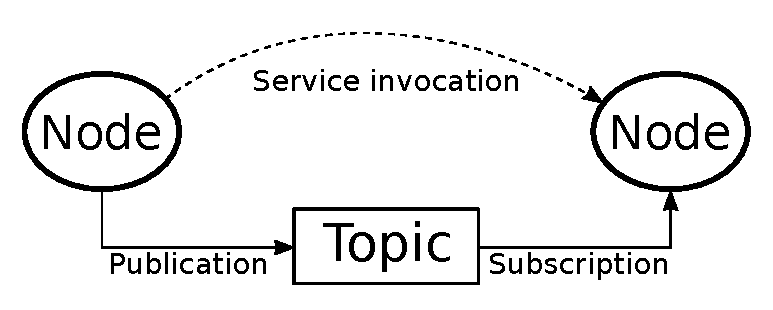
\includegraphics{Images/fig13-ros-basic-concept.eps}
    \caption[ROS basic concept]{ROS basic concepts. Two nodes communicate between them using the messages published in a topic. One node is responsible of publishing the topic, while the other subscribes and receives the messages of that particular topic. Furthermore, the node in the left calls a service provided by the node in the right, so that node will perform some computation and will return the result. \cite{ros-website}}
    \label{fig:chapter1:ros:basic_concepts}
\end{figure}

\subsection{Services}
\label{subsec:chapter1:ros:services}
As well as topics, services are a way to communicate nodes. The difference is that topics are an asynchronous way of communication, while services are synchronous. The key difference lies on the ability of nodes to decide when to trigger a service. Hence, services are used in between nodes to retrieve specific information or to request another node to carry out a computation beyond caller's node scope.


\subsection{Tools}
\label{subsec:chapter1:ros:tools}
Regarding the tools provided by ROS, one that is crucial for debugging and/or experimentation is the bag recording and playback. Since the exchange of messages between nodes is anonymous (meaning that nodes communicate between each others without knowing which node sent or received a message) it is possible to record the messages during a period of time, without taking into consideration which node sent a message and which node received it. This recorder bag is useful for debugging since it can be played back, hence reproducing a previous experiment. Also, it can be used for the development of new nodes that depend on the messages contained in the bag.\\

Another useful tool provided is \ac{RViz}, a 3D visualization tool. With this tool it is possible to see the robot, orientation, reference frames, covariance matrices, etc. In addition, it is possible to draw lines, arrows, text and others, onto the environment in order to see useful information that cannot be extracted from messages.

\subsection{MAVLink and MAVROS}
\label{sssec:chapter2:drone:mavlink}
%\nocite{mavlink}
MAVLink is a binary telemetry protocol designed for resource-constrained systems and bandwidth-constraint links, more specifically for drones of all kinds. As with ROS, it adopts a publisher-subscriber architecture, where data streams are published as topics. Its key features, as published in their website are:
\begin{itemize}
    \item Since its messages do not require any special framing, it is well suited for applications with very limited bandwidth.
    \item It provides methods for detecting package drops, corruption and for package authentication.
    \item Allows up to 255 concurrent systems on the network.
    \item Enables both offboard and onboard communications.
\end{itemize}
%\nocite{mavros}
MAVROS is the extension of MAVLink in ROS, with the additive of being a proxy for Ground Control Station tool. Its main features, as published in its website are:
\begin{itemize}
    \item Communication with autopilot via serial port, UDP or TCP .
    \item Internal proxy for Ground Control Station (serial, UDP, TCP).
    \item Plugin system for ROS-MAVLink translation.
    \item Parameter manipulation tool.
    \item Waypoint manipulation tool.
    \item PX4Flow support (by mavros\_extras).
    \item OFFBOARD mode support.
\end{itemize}

One characteristic that worth mentioning, is that it translates the \ac{NED} reference frames into \ac{ENU} reference frames, and vice-versa, so as to be compliant with ROS standard reference frames.

\subsection{RTAB-Map}
\label{subsec:chapter1:ros:octomap}
\ac{RTAB-Map} is a RGB-D, stereo and LiDAR graph-based \ac{SLAM} approach based on an incremental appearance-based loop closure detector. It allows to build a 3 dimensional map of the environment using a stereo camera, a LiDAR sensor and/or the odometry estimation. The map is built using a 3D occupancy grid by means of Octomap library, which builds a tree-based representation of the mapped area. Octomap library \enquote{performs a probabilistic occupancy estimation to ensure updatability and to cope with sensor noise}\cite{octomap-paper}.\\

The Octomap library generates an octotree, which is a hierarchical data structure used to generate spacial subdivision in 3 dimensions. Each node in an octotree represents a voxel, which is a cubic volume, which is at the same time, subdivided in eight smaller cubes until a given minimum voxel size called resolution. This way, the octotree data structure is used to build an occupancy grid of a volume. An example of a octotree can be seen in Figure~\ref{fig:chapter1:ros:octomap}, where the color of each occupied voxel represents its height: higher voxels are red-colored, while lower voxels are light-blue-colored.\\

\begin{figure}
    \centering
    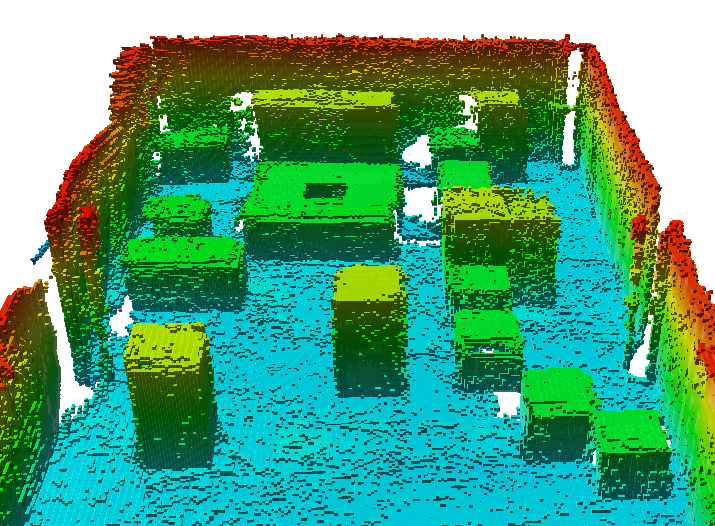
\includegraphics[width=\textwidth]{Images/fig14-octomap-colored2.png}
    \caption[Octomap example]{Octomap example. Octotree representation generated from data, showing occupied voxels only. \cite{octomap-paper}}
    \label{fig:chapter1:ros:octomap}
\end{figure}

RTAB-Map library, uses the Octomap library to store the 3D occupancy grid of the environment. The \inlinesrc{rtabmap_ros} node is the extension of the RTAB-Map library for ROS. It uses the information of the stereo camera or a RGB-D camera and/or a LiDAR information to create a cloud point that is used to build the map. Furthermore, it uses the provided odometry to estimate and correct the robot's pose into the 3D map. An example of this procedure can be seen in Figure~\ref{fig:chapter1:ros:rtabmap}.

\begin{figure}
    \centering
    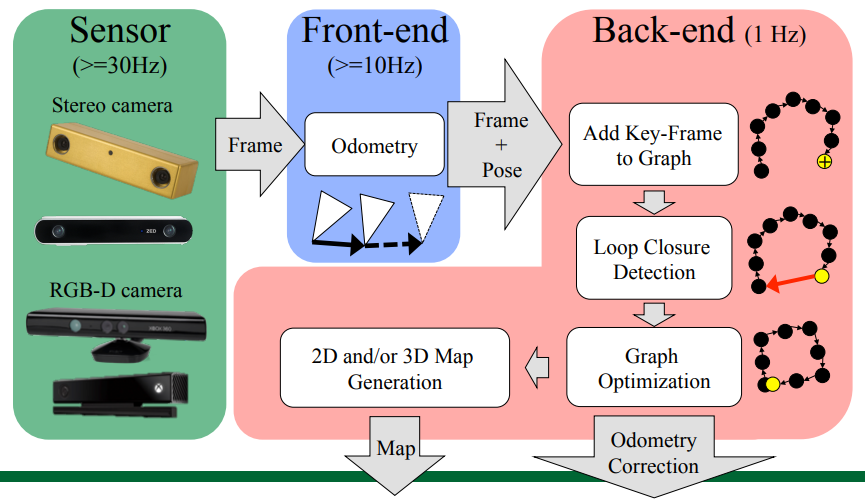
\includegraphics[width=\textwidth]{Images/fig14-rtabmap3.png}
    \caption[RTAB-Map example]{RTAB-Map example. An stereo camera or a RGB-D camera is used among the odometry estimation. Both are used to generate a 3D occupancy grid using Octomap library, and to correct the odometry estimation. \cite{rtabmap-presentation}}
    \label{fig:chapter1:ros:rtabmap}
\end{figure}

\section{Transformations}
\label{sec:chapter1:transform}
A robot, in this case the drone, can be considered as a rigid body that moves and rotates around the environment. Hence, it is necessary to model the drone displacement in space, and this can be done by decomposing the movement as translations and rotations.

\subsection{Translation}
\label{subsec:chapter1:transform:translation}
Given a vector $\bm{b} = \begin{bmatrix}b_x & b_y & b_z\end{bmatrix}^T$ that represents the center of mass of a rigid body, a translation that displaces $\bm{b}$ parallel to itself of a given vector $\bm{t}$ can be defined as:
\begin{align*}
    \bm{b} + \bm{t} = \begin{bmatrix}
        b_x \\ b_y \\ b_z
    \end{bmatrix} + \begin{bmatrix}
    t_1 \\ t_2 \\ t_3
\end{bmatrix} = \begin{bmatrix}
        b_x + t_1\\ b_y + t_2 \\ b_z + t_3
\end{bmatrix}
\end{align*}
Given a point $\mathcal{P}$ represented in the reference frame $\mathcal{R}_m$ by $\bm{v_P^m}$ will be represented in the reference frame $\mathcal{R}_n$ by:
\begin{align*}
    \bm{v_P^n} = \bm{v_P^m} + \bm{t_m^k}
\end{align*}

\subsection{Rotation}
\label{subsec:chapter1:transform:rotation}
In three dimensional space, any displacement of a rigid body is equivalent to a single rotation of a given angle about some axis that contains the point. It is possible to express the previous statement as $\bm{v} = \bm{u} * \theta$, being $\bm{u}$ a unit vector representing the axis and $\theta$ the angle.\\

Unlike with translations, two or more rotations cannot be simply the sum of the related vectors. A rotation can be described assuming a rigid body in a reference frame with its origin fixed, while the unit vectors are changed under the rotation. This way, a rotation is characterized by the mathematical relation of these two reference frames. Hence, in order to represent a rotation, two reference frames with a common origin are needed, as shown in Figure~\ref{fig:chapter1:transformation:rotation:3d-example}. At the beginning the two reference frames coincide, then one of them is rotated around the origin by an arbitrary angle. After this procedure, the two reference frames are not coincident anymore, however, both share the same origin.\\

\begin{figure}
    \centering
    \includegraphics[width=\textwidth]{Images/fig17-3D-rotation-example}
    \caption[Rotation around origin]{Rotation around origin. The reference frame at the left is rotated around Y axis and, as result, a new reference frame is obtained, both sharing the same origin.}
    \label{fig:chapter1:transformation:rotation:3d-example}
\end{figure}

The rotation by any angle of any axis can be represented in a matrix form, $\bm{R_n^m}$, where each column of the matrix represents the unit vector of $R_n$ in $R_m$, so it represents the rotated frame $R_n$ with respect the fixed frame $R_m$ with common origin. Furthermore, it is possible to show that matrix $\bm{R_n^m}$ is \emph{orthonormal}, which means that its inverse is equal to its transpose.\\

Given the matrix representation of a rotation, it is possible to provide a way to rotate a vector in the space. When the reference frames origins are the same, the rotation of a vector is possible by multiplying it by the rotation matrix around an axis: $\bm{v^m} = \bm{R_n^m} \bm{v^n}$. This kind of rotations are called \emph{elementary rotations}, and given that there are three axis in a 3D space, three different elementary rotations can be defined:
\begin{enumerate}
    \item{Rotation around axis $x$: \begin{align*}
            \bm{R_{x, \theta}} = \begin{bmatrix}
                1 & 0 & 0 \\ 0 & \cos{\left(\theta\right)} & -\sin{\left(\theta\right)} \\ 0 & \sin{\left(\theta\right)} & \cos{\left(\theta\right)}
            \end{bmatrix}
    \end{align*}}
    \item{Rotation around axis $y$: \begin{align*}
        \bm{R_{y, \theta}} = \begin{bmatrix}
             \cos{\left(\theta\right)} & 0 &  \sin{\left(\theta\right)} \\ 0 & 1 & 0 \\  -\sin{\left(\theta\right)} & 0 & \cos{\left(\theta\right)}
        \end{bmatrix}
    \end{align*}}
    \item{Rotation around axis $y$: \begin{align*}
        \bm{R_{z, \theta}} = \begin{bmatrix}
            \cos{\left(\theta\right)} & -\sin{\left(\theta\right)} & 0 \\ \sin{\left(\theta\right)} & \cos{\left(\theta\right)} & 0 \\ 0 & 0 & 1
        \end{bmatrix}
    \end{align*}}
\end{enumerate}

As mentioned, unlike translations, rotations cannot be summed. Hence, if two consecutive rotations need to be performed around two axis, a multiplication is needed:
\begin{align}
    \bm{R_{y,x}} = \bm{R_{x, \alpha}} * \bm{R_{y, \beta}}
\end{align}
where $\bm{R_{y,x}}$ is the rotation around axis $y$ by an angle $\beta$ followed by a rotation around the new axis $x$ by an angle $\alpha$, as shown in Figure~\ref{fig:chapter1:transform:rotation_z_x}.

\begin{figure}
    \centering
    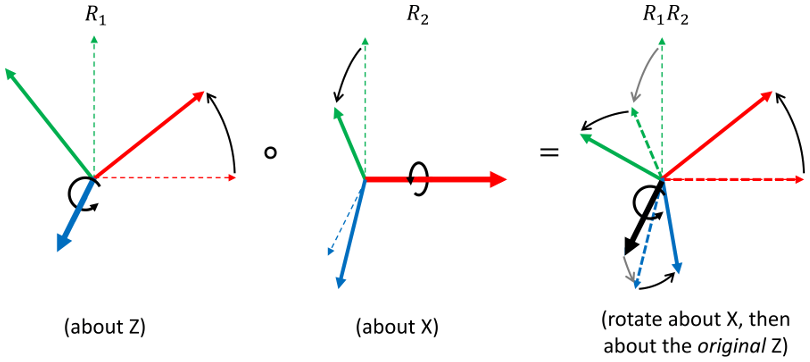
\includegraphics[width=\textwidth]{Images/fig16-rotations.png}
    \caption[Rotation around axis $z$ followed by rotation about axis $x$]{Rotation about axis $z$ followed by rotation about axis $x$. The second rotation is performed about the original axis $z$. This final rotation can be achieve by multiplying $R_1$ and $R_2$.\cite{hauser-robotics-systems}}
    \label{fig:chapter1:transform:rotation_z_x}
\end{figure}

\subsection{Homogeneous Transform}
\label{subsec:chapter1:transform:rototranslation}
A rotation and a translation can be accomplished as follow: $\hat{\bm{v}} = \bm{R}\bm{v} + \bm{t}$. Nevertheless, this can be achieve by using \emph{homogeneous coordinates}, where the point $\bm{v}$, expressed in its homogeneous representation, is $\bm{v} = \begin{bmatrix}v_x & v_y & v_z & 1\end{bmatrix}^T$. This way, the rotation and translation of a point can be accomplished by multiplying the 3D point with the homogeneous transformation matrix:
\begin{align}
    \bm{T}_m^n &= \begin{bmatrix}
        \bm{R}_m^n & \bm{t} \\
        \bm{0} & 1
    \end{bmatrix}
    \label{eq:chapter1:transform:homogeneous_transform}\\
    \hat{\bm{v}}^n &= \bm{T}_m^n\bm{v}^m
\end{align}
As can be noticed in equation~(\ref{eq:chapter1:transform:homogeneous_transform}), the homogeneous transformation is represented by a $4 \times 4$ matrix, and unlike the pure rotation matrix showed in Section~\ref{subsec:chapter1:transform:rotation}, the inverse of the homogeneous transformation is not equal to its transpose. The inverse of the homogeneous transformation is equivalent to:
\begin{align}
    \bm{T}^{-1} &= \begin{bmatrix}
        \bm{R}^T & -\bm{R}^T\bm{t} \\
        \bm{0} & 1
    \end{bmatrix}
\end{align}

\begin{figure}
    \centering
    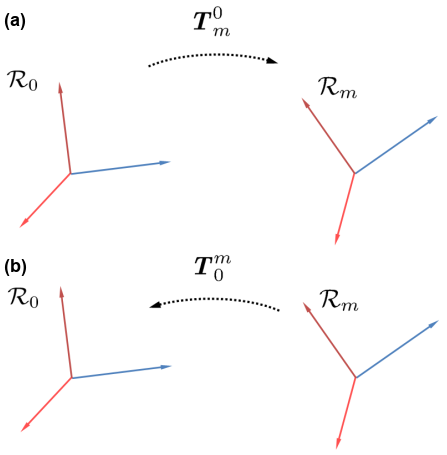
\includegraphics[width=0.5\textwidth]{Images/fig15-homogeneous-transform.png}
    \caption[Example of a Homogeneous transform]{Example of a Homogeneous transform. \textbf{(a)} Transformation $\bm{T}_m^0$ is applied to a point in reference frame $\mathcal{R}_0$ to express it in reference frame $\mathcal{R}_m$. \textbf{(b)} The inverse transformation is applied, so to express the point in reference frame $\mathcal{R}_m$ into reference frame $\mathcal{R}_0$.  \cite{bona-dynamic-modelling}}
    \label{fig:chapter1:transform:homogeneous}
\end{figure}

\section{Kalman Filter}
\label{sec:chapter1:kf}
%\nocite{intro-robotics}

Introduced by \cite{kalman}, the \ac{KF} provides a recursive method for estimating the state of a dynamic system with presence of noise. It is a technique for filtering and prediction in \emph{linear Gaussian systems} and applicable only to continuous states. One of its key features is that it simultaneously maintains estimates of the state vector and the estimate error covariance. It assures that the posteriors are Gaussian if the Markov assumption is hold, in addition to three conditions. The Markov assumption states that the past and future data are independent if one knows the current state; the other three conditions are the following:
\begin{enumerate}
    \item{The state transition probability $p\left( x_t | u_t, x_{t-1}\right)$ must be a linear function in its arguments. This is guaranteed by $ x_t = A_t x_{t-1} + B_t u_t + \epsilon_t $. Here, $x_t$ and $x_{t-1}$ are the state vectors, of size $n$, and $u_t$ represents the control vector, of size $m$, at time $t$; $A_t$ and $B_t$ are matrices of size $n \times n$ and $n\times m$ respectively. In this way, the state transition function becomes linear in its arguments, hence KF assumes a linear system dynamics. \\\\ $\epsilon_t$ represents the uncertainty introduced by the state transition, and it is a Gaussian random variable with zero mean and $R_t$ covariance.}
    \item{The measurement probability $p\left(z_t | x_t\right)$ must be linear in its arguments. This is guaranteed by $z_t = C_t x_t + \delta_t$, where $z_t$ represents the measurement vector of size $k$, $C_t$ is a matrix of size $k \times n$ and $\delta_t$ is a Gaussian noise with zero mean and $Q_t$ covariance.}
    \item{The initial belief should be normally distributed.}
\end{enumerate}
Given these three conditions, we are guaranteed that the posterior probability is Gaussian.

\begin{algorithm}[h]
    \caption{Kalman Filter algorithm}
    \label{alg:chapter1:kf}

    \BlankLine
    \KwIn{$\mu_{t-1}$, $\Sigma_{t-1}$, $u_t$, $z_t$}
    \BlankLine
    $\hat\mu_t = A_t \mu_{t-1} + B_t u_t$ \\
    $\hat\Sigma_t = A_t \Sigma_{t-1} A_t^T + R_t$ \\
    \BlankLine
    $K_t = \hat\Sigma_t C_t^T \left(C_t \hat\Sigma_t C_t^T + Q_t\right)^{-1}$ \\
    $\mu_t = \hat\mu_t + K_t \left(z_t - C_t \hat\mu_t \right) $ \\
    $\Sigma_t = (I - K_t C_t) \hat\Sigma_t$ \\
    \BlankLine
    \Return{$\mu_t$, $\Sigma_t$}
\end{algorithm}

The KF can be seen in Algorithm~\ref{alg:chapter1:kf} and its input is the belief at time $t-1$, represented by its mean ($\mu_{t-1}$) and its covariance ($\Sigma_{t-1}$), in addition to the control vector ($u_t$) and the observations ($z_t$). As a result, it returns the current belief characterized by its mean $\mu_t$ and covariance $\Sigma_t$. \\

The first step in the algorithm (lines 1 and 2), represent the prediction step. It calculates the current belief before incorporating the observations, but after adding the control vector. The estimated belief is characterized by its mean, $\hat\mu_t$ , and its covariance $\hat\Sigma_t$.\\

The second step (from line 3 to 5) starts by calculating $K_t$, the Kalman gain, which specifies the degree in which the observation is incorporated to the new state estimate. $K_t$ can be seen as the weighting factor that weights the relationship between the accuracy of the predicted state estimate and the observation noise. When $K_t$ is large, the observations have more importance in the final estimate; while if $K_t$ is small, the observations do not have much importance in the correction step. Following, at line 4, the new mean is estimated by means of the Kalman gain and the \emph{innovation}, which is the difference between the observation $z_t$ and the expected measurement $C_t \hat\mu_t$. Finally, the new covariance is calculated.

\subsection{Extended Kalman Filter}
\label{subsec:chapter1:kf:ekf}

The linearity conditions that make the KF to work are, in some cases, far from reality: state transition functions and measurements are rarely linear in practice. The \ac{EKF} works through a process of linearization, where nonlinear state transition and observation functions are approximated by a Taylor series expansion. \\

\begin{figure}
    \centering
    \includegraphics[width=\textwidth]{Images/fig1-kf-ekf.png}
    \caption[Linear and nonlinear transformation of a Gaussian random variable]{Linear \textbf{(a)} and nonlinear \textbf{(b)} transformation of a Gaussian random variable. The lower right plot shows the density function of the random variable. The upper right plot shows the transformation of the random variable. The upper left plot shows the resulting density function. \cite{prob-robotics}}
    \label{fig:chapter1:kf:ekf:cmp-kf-ekf}
\end{figure}

The Figure~\ref{fig:chapter1:kf:ekf:cmp-kf-ekf}a shows the linear transformation of a random Gaussian variable, whose density function is $\mathcal{N}\left(x; \mu, \sigma^2 \right)$. Assuming that the random variable is transformed using a linear function $y = ax + b$, the resulting random variable will be Gaussian with mean $a\mu + b$ and variance $a^2 \sigma^2$.\\

However, as shown in Figure~\ref{fig:chapter1:kf:ekf:cmp-kf-ekf}b, this does not happen if the transformation is not linear. In this case, assuming the original random variable is transformed using a nonlinear function $g$, the density of the resulting random variable is not Gaussian anymore.\\

The state transition probability and observation probabilities are ruled by nonlinear functions $g$ and $h$ respectively. Matrices $A$ and $B$ are replaced by function $g\left(u_t, x_{t-1}\right)$ and matrix $H$ is replaced by function $h \left(x_t\right)$, making the belief not Gaussian. This is solved in EKF by approximating to the true belief, not the exact one as happens with linear KF. The approximation is done using a linearization method that approximates the nonlinear function by a linear function that is tangent to it, thereby maintaining the Gaussian properties of the posterior belief. \\

The used method is the first order Taylor expansion, which constructs a linear approximation of a function $g$ from $g$'s value and slope, which is given by
\begin{equation}
    g' \left(u_t, x_{t-1}\right) = \frac{\partial g\left(u_t, x_{t-1}\right)}{\partial x_{t-1}}
    \label{eq:chapter1:kf:ekf:g-derivative}
\end{equation}

 Since $g$ depends on the control variable $u$ and the state $x$, we need to define a value for $x$, and the logical choice is the mean of the posterior in the previous time step: $\mu_{t-1}$. This way
 \begin{equation}
    g \left(u_t, x_{t-1}\right) = g \left(u_t, \mu_{t-1}\right) + g' \left(u_t, \mu_{t-1}\right)\left(x_{t-1} - \mu_{t-1}\right)
    \label{eq:chapter1:kf:ekf:g-mean-cov}
 \end{equation}
where $g'$ is the \emph{Jacobian} of $g$, usually expressed as $G_t$, and it depends on $u_t$ and $\mu_{t-1}$, hence it changes through time.\\

The same linearization is applied to the observation function $h$:
\begin{equation}
    h\left(x_t\right) = h\left(\hat\mu_t\right) + h'\left(\hat\mu_t\right)\left(x_t - \hat\mu_t\right)
\end{equation}
\begin{equation}
        h'\left(\hat\mu_t\right) = \frac{\partial h\left(x_t\right)}{\partial x_t}
\end{equation}
where $h'$ is the Jacobian of $h$, usually expressed as $H_t$. In this case, the linearization is done around $\hat\mu_t$, which is the state estimate just before computing $h$.\\

\begin{figure}[h]
    \centering
    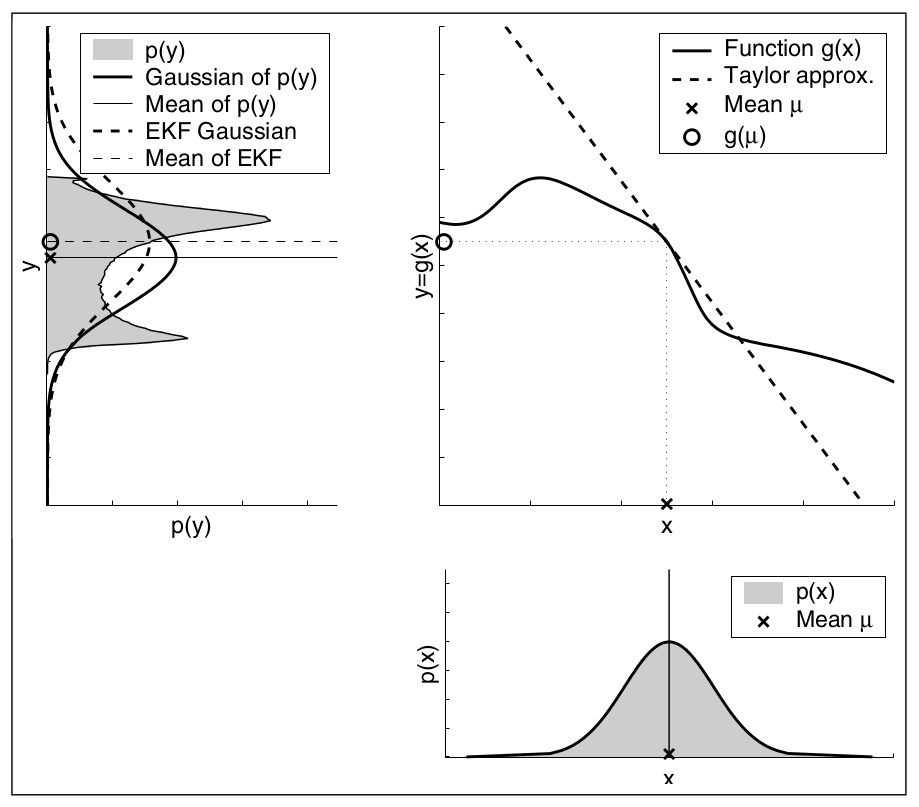
\includegraphics{Images/fig2-ekf-linearization.png}
    \caption[Linearization applied in EKF]{Linearization applied in EKF. In this case, the nonlinear function $g$ is approximated using first order Taylor expansion, that is a linear function tangent to $g$ at the mean of the original density function. The linearization is not perfect, so it adds an error, depicted in the upper left plot. This error is the difference between the dashed line and the solid line. \cite{prob-robotics}}
    \label{fig:chapter1:kf:ekf:ekf-linearization}
\end{figure}

The Figure~\ref{fig:chapter1:kf:ekf:ekf-linearization} depicts the approximation of $g$ by a linear function that is tangent around its mean. The resulting density function is shown in the upper left plot with a dashed line, that is similar to the original density function.\\

\begin{algorithm}[h]
    \caption{Extended Kalman Filter algorithm}
    \label{alg:chapter1:kf:ekf}

    \BlankLine
    \KwIn{$\mu_{t-1}$, $\Sigma_{t-1}$, $u_t$, $z_t$}
    \BlankLine
    $\hat\mu_t = g \left(u_t, \mu_{t-1}\right)$ \\
    $\hat\Sigma_t = G_t \Sigma_{t-1} G_t^T + R_t$ \\
    \BlankLine
    $K_t = \hat\Sigma_t H_t^T \left(H_t \hat\Sigma_t H_t^T + Q_t\right)^{-1}$ \\
    $\mu_t = \hat\mu_t + K_t \left(z_t - h \left(\hat\mu_t\right) \right) $ \\
    $\Sigma_t = (I - K_t H_t) \hat\Sigma_t$ \\
    \BlankLine
    \Return{$\mu_t$, $\Sigma_t$}
\end{algorithm}

The EKF algorithm can be seen in Algorithm~\ref{alg:chapter1:kf:ekf}, and it is similar to Algorithm~\ref{alg:chapter1:kf}. The difference lies in the usage of the nonlinear functions $g$ and $h$ and their Jacobians, $G_t$ and $H_t$ respectively.

\section{Simultaneous Localization and Mapping}
\label{sec:chapter1:slam}
Among all the problems faced by autonomous mobile robots, two of them are relevant for this work: localization and mapping. The former one, is related to the problem of where the robot is, while the later is related to building a map of the environment. However, in order to accurately localize itself the robot needs a map of the environment in which it is immersed in, and, in order to build a map, it needs to know where it currently is, giving us a chicken-egg situation. Hence, the \ac{SLAM} problem appears when the robot has no knowledge of its localization nor its environment map, while measurements and controls are given.\\

The problem of building a map can be summarized in the following steps:
\begin{enumerate}
    \item{The robot senses the environment using its sensors}
    \item{It creates a representation of the acquired data}
    \item{It integrates the processed sensor data with the previously learned map structure}
\end{enumerate}

While this process can be done by manually moving the robot around the environment, it is more challenging to build the map while the robot is moving autonomously. \\

%\nocite{intro-aut-mobile-robots}
On the other hand, assuming that the robot already knows the map, the localization problem could be trivial if no noise is present at all. The sensors, wheel encoders, different kinds of terrain, battery life, etc, all of these can make the robot to increase its uncertainty related to where it is. As robot moves around the environment it uses its sensors to estimate its position, increasing its uncertainty regarding its position relative to the map. At some point, the robot will "see" a known landmark or feature in the environment, correcting its position while reducing the uncertainty.\\
\begin{figure}
    \centering
    \includegraphics[width=\textwidth]{Images/fig3-slam.png}
    \caption[Example of SLAM problem]{At the beginning \textbf{(a)} the robot has low uncertainty regarding its pose. As it moves around the environment its uncertainty, represented by the dark gray ellipsis, grows \textbf{(b), (c), (d)}, until it sees a known landmark \textbf{(e)}, making the position uncertainty to shrink. \cite{intro-aut-mobile-robots}}
    \label{fig:chapter1:slam}
\end{figure}

The localization and mapping problems can be solved together by using a SLAM technique, with which the robot will build the map while localizing itself in it. An example of this problem can be seen in Figure~\ref{fig:chapter1:slam}, where a robot moves around the environment and sees some features or landmarks. The uncertainty regarding its position is low when it starts, and keeps growing while it moves around. At the end, it sees a known landmark ($m_0$) making the uncertainty to shrink. As can be seen in the figure, the robot adds new landmarks to the map ($m_1$ and $m_2$) with their corresponding uncertainty, and when the robot sees the first landmark, not only its own uncertainty decreases, but also the two new landmarks' uncertainty. In this way, the robot's position is correlated with the observations' position estimates.\\

The idea of the SLAM problem is to estimate a posterior belief that involves not only the robot pose, but also the map: $p\left(x_t, m | z_{1:t}, u_{1:t}\right)$, where $x_t$ is the robot's pose at time $t$, $m$ is the map, $z_{1:t}$ are the measurements, and $u_{1:t}$ are the controls given to the robot.

\subsection{EKF-SLAM}
\label{subsec:chapter1:slam:ekfslam}
The SLAM problem can be addressed, between others, using an EKF approach. The algorithm proceeds in the same way as shown in Section~\ref{subsec:chapter1:kf:ekf}, being $\mu$ a state vector containing the information for the robot pose ($q_r$) and the landmarks' pose ($m_i$):
\begin{equation}
    \mu = \begin{bmatrix}
        q_r & m_0 & \dots & m_{n-1}
    \end{bmatrix}^T
\end{equation}

One thing that is worth mentioning is that in EKF-SLAM maps are \emph{feature based}. This means that the features or landmarks are assumed to be points in the space: if the robot sees, for example, a chair, it will store a point that represents the chair in space. Also, as explained before, it assumes Gaussian noise for the robot motion and observations.\\

The EKF-SLAM algorithm estimates the robot's pose in addition to all encountered landmarks' poses along its way. Thus, there is a correspondence between robot's pose and landmarks, and that is why it is necessary to include the landmarks information into the state vector. Hence, the algorithm estimates the posterior $p\left(\mu_t | z_t, u_t\right)$.\\

\begin{algorithm}[h]
    \caption{EKF-SLAM algorithm}
    \label{alg:chapter1:slam:ekfslam}
    \BlankLine
    \KwIn{$\mu_{t-1}$, $\Sigma_{t-1}$, $u_t$, $z_t$}
    \BlankLine
    $\hat\mu_t = g\left(\mu_{t-1}, u_t\right)$\;
    $G_t = computeJacobian\left(g\right)$\;
    $\hat\Sigma_t = G_t \Sigma_{t-1} G_t^T + R_t$\;
    \BlankLine
    \ForEach{landmark observation $z_t^i$}{
        \BlankLine
        \If{landmark $i$ has not being seen before}{
            $addLandmarkToStateVector\left( z_t^i \right)$
        }
        \BlankLine
        $H_t^i = computeJacobian\left( h^i \right)$\;
        $v^i =  z_t^i - h^i \left( \hat\mu_t \right)$\;
        $S = H_t^i \hat\Sigma_t H_t^{iT} + Q_t$\;
        $K_t^i = \hat\Sigma_t H_t^{iT} S^{-1}$ \;
        $\mu_t = \hat\mu_t + K_t^i \left( v^i \right) $ \;
        $\Sigma_t = (I - K_t^i H_t^i) \hat\Sigma_t$ \;
    }
    \BlankLine
    \Return{$\mu_t$, $\Sigma_t$}
\end{algorithm}

Assuming the robot's pose is composed by $x$, $y$, $\theta$ , the markers' pose is composed by $x$, $y$, and there are $N$ markers, the state vector $\mu$ will have a length of $3 \times 2N$, and the covariance matrix $\Sigma$ will have a size of $(3 \times 2N) \times (3 \times 2N)$.\\

The algorithm can be seen in Algorithm~\ref{alg:chapter1:slam:ekfslam}. From lines 1 to 3, it computes the state vector and covariance matrix updates; the function $computeJacobian$ computes, indeed, the Jacobian matrix for the motion model $g$, and the resulting matrix has the same size as the covariance matrix and has the following characteristic:
\begin{align}
   G_t &= \begin{bmatrix}
        G_r & \textbf{0} \\
        \textbf{0} & \textbf{I}
    \end{bmatrix}\\
    G_r &= \begin{bmatrix}
    \frac{\partial x'}{\partial \mu_{t-1,x}} & \frac{\partial x'}{\partial \mu_{t-1,y}} & \frac{\partial x'}{\partial \mu_{t-1,\theta}}\\
    \frac{\partial y'}{\partial \mu_{t-1,x}} & \frac{\partial y'}{\partial \mu_{t-1,y}} & \frac{\partial y'}{\partial \mu_{t-1,\theta}}\\
    \frac{\partial \theta'}{\partial \mu_{t-1,x}} & \frac{\partial \theta'}{\partial \mu_{t-1,y}} & \frac{\partial \theta'}{\partial \mu_{t-1,\theta}}
\end{bmatrix}
\end{align}
where $\frac{\partial x'}{\partial \mu_{t-1,x}}$ is the derivative of $g$ along $x'$ dimension, taken with respect to $x$, $y$.. at $\mu_{t-1}$.\\

At line 4, it iterates through every observation $z_t$. At each time step $t$, a sensor obtains a set of observations $z^i$ of one of the $N$ landmarks. Each observation is associated with a map feature, and this association is accomplished by a prediction of the measurement that each feature would generate and a measure of the difference between the prediction and the sensor measurement. The prediction of the measurements can be obtained by the observation model $h^i$, which result is a vector of predicted features. If the observation $z^i$ comes from a landmark $i$, the following relation is hold:
\begin{align}
    z^i = h^i\left(x_t\right) + w^i
\end{align}
where $x_t$ is the true state and $w^i$ is the observation noise with covariance $Q_t$, and assumed to be zero mean, Gaussian, additive and independent of the process noise. If the landmark is not already in the state vector, at line 6 it is added by projecting the observation and calculating the landmark's pose, adding two new elements to the state vector and two new more columns and rows to the covariance matrix. At line 7 the Jacobian of the observation model is computed.\\

At line 8, the innovation is calculated while its covariance is calculated at line 9. The innovation measures the discrepancy between the predicted observation and the actual sensor measurement. At line 10 the Kalman gain is computed, and at line 11 the state vector is updated. The gain propagates the information through all the state vector, updating not only the robot's pose, but also the landmarks' poses.\\

The fact that the Kalman gain is not sparse is important, because observing a landmark not only improves the estimate of that landmark's pose, but also all the others, along with the robot's pose. This effect can be seen in Figure~\ref{fig:chapter1:slam}, with an additional explanation: most of the uncertainty of the landmarks' poses is caused by the robot's own uncertainty, so the location of those previously seen landmarks are correlated. When the robot gains information about its own pose, this information is propagated to the landmarks, and as result it improves the localization of other landmarks in the map.

\subsection{Adding new landmarks}
\label{subsec:chapter1:slam:ekfslam:addlandmarks}
So far, the existence and accuracy of a map was assumed. Nevertheless, this is not always true, and the construction of a map should somehow be done. Hopefully, EKF-SLAM algorithm considers the possibility of adding new landmarks to the map while doing the localization process with known landmarks. This process of adding new landmarks to the map is done via what is called inverse observation model, which handles the sensor measurements, identifies the new landmark, and adds it to the state vector.\\

The inverse observation model will produce the coordinates of the new landmark in the map, and this information will be added to the state vector, which will increase its size (in this case) by two new elements.
\begin{align}
    h^{-1}\left(\bm{x_r}, \bm{z}\right) &= \begin{bmatrix}
        x_l \\ y_l
    \end{bmatrix}
    \label{eq:chapter1:slam:ekfslam:inverseh}\\
    \bm{x_t} = y\left(\bm{x}, \bm{z}\right) &= \begin{bmatrix}
        \bm{x} \\ h^{-1}\left(\bm{x_r}, \bm{z}\right)
    \end{bmatrix}
    \label{eq:chapter1:slam:ekfslam:extension_y}
\end{align}
In equation~(\ref{eq:chapter1:slam:ekfslam:inverseh}) $\bm{x_r}$ refers to the elements in the state vector that corresponds to the robot's pose, and $\bm{z}$ refers to the observation elements, which can be, for example, range and bearing data. Since the state vector has a variable length, extending the covariance matrix is also needed whenever the robot sees a landmark that has not being seen previously. The extension of the covariance matrix is achieved as shown in equation~(\ref{eq:chapter1:slam:ekfslam:cov_update}).
\begin{align}
    \hat{\bm{\Sigma}} = \bm{Y_x} \bm{\Sigma} \bm{Y_x}^T + \bm{Y_z} \bm{Q}_t \bm{Y_z}^T
    \label{eq:chapter1:slam:ekfslam:cov_update}\\
    \bm{Y_x} = \frac{\partial y}{\partial x} = \begin{bmatrix}
        \frac{\partial x}{\partial x} \\ \frac{\partial h^{-1}}{\partial x}
    \end{bmatrix} = \begin{bmatrix}
    \bm{I} \\ \bm{G_x}
    \end{bmatrix}
    \label{eq:chapter1:slam:ekfslam:yx}\\
    \bm{Y_z} = \frac{\partial y}{\partial z} = \begin{bmatrix}
        \frac{\partial x}{\partial z} \\ \frac{\partial h^{-1}}{\partial z}
    \end{bmatrix} = \begin{bmatrix}
        \bm{0} \\ \bm{G_z}
    \end{bmatrix}
    \label{eq:chapter1:slam:ekfslam:yz}
\end{align}
where matrices $\bm{Gx}$ and $\bm{Gz}$ are the Jacobian of function $h^{-1}$ with respect to the state vector and the observation vector respectively. By substituting the Jacobians in equations (\ref{eq:chapter1:slam:ekfslam:yx}) and (\ref{eq:chapter1:slam:ekfslam:yz}) into equation~(\ref{eq:chapter1:slam:ekfslam:cov_update}), the following matrix is obtained:
\begin{align}
    \hat{\bm{\Sigma}} = \begin{bmatrix}
        \bm{\Sigma} & \bm{\Sigma} \bm{G_x}^T \\
        \bm{G_x} \bm{\Sigma} & \bm{G_x} \bm{\Sigma} \bm{G_x}^T + \bm{G_z} \bm{Q}_t \bm{G_z}^T
    \end{bmatrix}
    \label{eq:chapter1:slam:ekfslam:cov_update_full}
\end{align}\\

The linearized covariance update can be factored as shown in equation~(\ref{eq:chapter1:slam:ekfslam:factoring}) by assuming that $A \equiv 1$, $B \equiv 0$, $C \equiv 0$ and $D \equiv \bm{G_z}$
\begin{align}
    \begin{bmatrix}
        A & B \\ C & D
    \end{bmatrix} \begin{bmatrix}
        P & 0 \\ 0 & Q
    \end{bmatrix} \begin{bmatrix}
        A & B \\ C & D
    \end{bmatrix}^T &= \begin{bmatrix}
            APA^T + BQB^T & APC^T + BQD^T \\
            CPA^T + DQB^T & CPC^T + DQD^T
    \end{bmatrix}
    \label{eq:chapter1:slam:ekfslam:factoring}\\
    \hat{\bm{\Sigma}} &= \begin{bmatrix}
        \bm{1} & \bm{0} \\ \bm{G_x} & \bm{G_z}
    \end{bmatrix} \begin{bmatrix}
        \bm{\Sigma} & \bm{0} \\ \bm{0} & \bm{Q}_t
    \end{bmatrix} \begin{bmatrix}
        \bm{1} & \bm{0} \\ \bm{G_x} & \bm{G_z}
    \end{bmatrix}^T
    \label{eq:chapter1:slam:ekfslam:factored_cov_update}\\
\end{align}

\section{Normalized Estimation Error Squared}
\label{sec:chapter2:nees}
The Mahalanobis distance is a measure of the distance between a point and a distribution. It is a way to measure how many standard deviations is away the point from the mean of the distribution. The Mahalanobis distance of an observation $\bm{x} = \begin{bmatrix}x_1 & x_2 & \dots \end{bmatrix}$ with mean $\bm{\mu} = \begin{bmatrix}\mu_1 & \mu_2 & \dots \end{bmatrix}$, and covariance matrix $\Sigma$ is defined as:
\begin{equation}
    D = \sqrt{\left(\bm{x} - \bm{\mu}\right) \Sigma^{-1} \left(\bm{x} - \bm{\mu}\right)}
\end{equation}\\
Every time the drone observes a pole or a marker, a node responsible of identifying the landmark processes the features that distinguish it with respect to other landmarks, and publishes these features as a message. In the case of poles, the message type is \inlinesrc{RangeAndBearingPole}, which contains the range and bearing information, and in the case of markers the message type is \inlinesrc{Pose}, which contains the position and orientation information of the observed marker. Given this, each observation $z$ for a pole, is composed by three measurements, and each observation of a marker is composed by six measurements. After observing a landmark the Algorithm~(\ref{alg:chapter1:slam:ekfslam}) calculates the discrepancy between the observation $i$ and the predicted observation by the innovation ($v^i$), and its covariance ($S$), as
\begin{align*}
    v^i =  z_t^i - h^i \left( \hat\mu_t \right)\\
    S = H_t^i \hat\Sigma_t H_t^{iT} + Q_t
\end{align*}

The square of the Mahalanobis distance can be used in order to establish a correspondence between the observed measurements with the landmark features if the following is hold:
\begin{align}
    D_i^2 = v^i S^{-1} v^i < \chi_{d, 1-\alpha}^2
    \label{eq:chapter2:nees:innov_test}
\end{align}
where $d$ is the size of $h^i$ and $1-\alpha$ is the desired confidence level. This test is called individual compatibility, and when applied to the predicted state can be used to determine the subset of observation features that are compatible with the observation.\\

Furthermore, a state estimate is consistent if its state estimation error $\bm{x} - \hat{\bm{x}}$ satisfies
\begin{align*}
    \mathbb{E}\left[\bm{x} - \hat{\bm{x}}\right] = 0\\
    \mathbb{E}\left[\left(\bm{x} - \hat{\bm{x}}\right)\left(\bm{x} - \hat{\bm{x}}\right)^T\right] \le \Sigma
\end{align*}
When the ground truth $\bm{x}$ is available, a \ac{NEES} can be performed to check the consistency of the filter. NEES test can be defined as the squared Mahalanobis distance for the difference between $\bm{x}$ and $\hat{\bm{x}}$, and consistency can be checked with a $\chi^2$ test
\begin{align*}
    NEES = \left(\bm{x} - \hat{\bm{x}}\right) \Sigma^{-1} \left(\bm{x} - \hat{\bm{x}}\right) \le \chi_{d, 1-\alpha}^2
\end{align*}

However, the ground truth is only available in simulated environments thus, the consistency of the filter is maintained by using observations that satisfy the test in equation~(\ref{eq:chapter2:nees:innov_test}). This way, the filter will discard observations that do not satisfy the innovation test, maintaining a consistent estimation of the state and therefore, the map.
 % Include the first content chapter
%\chapter{EKF-SLAM Implementation}
\label{ch:chapter2}
In Chapter~\ref{ch:chapter1} the EKF-SLAM algorithm in the context of SLAM was explained. As mentioned in Section~\ref{sec:chapter1:kf}, the algorithm can be summarized in two steps: prediction and correction. In the first stage involves the prediction of the next state of the system, meanwhile, during the correction stage, this estimation is updated. \\

In this chapter, an EKF-SLAM implementation is shown, starting from the used drone characteristics, going through the prediction and correction steps, and ending with the overall system's architecture.

\section{The Drone}
\label{sec:chapter2:drone}
\subsection{Characteristics}
\label{subsec:chapter2:drone:characteristics}
The drone considered for this analysis has a common characteristics, such as four rotors disposed as an X. The drone frame is called 3DR Iris Quadrotor, and can be seen in Figure~\ref{fig:chapter2:drone:frame}. Its total weight is XX kg., and it diameter is XX cm.\\

\begin{figure}
    \centering
    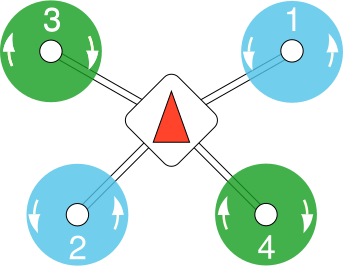
\includegraphics[width=0.5\textwidth]{Images/fig4-quad-frame.png}
    \caption{3DR Iris Quadrotor frame.}
    \label{fig:chapter2:drone:frame}
\end{figure}

\subsubsection{Flight Controller}
The flight controller used in this case is a PixHawk 4, and its characteristics are shown in Table~\ref{tab:chapter2:drone:px4fc}. It is worth mentioning that it includes an integrated accelerometer, a gyroscope, a magnetometer and a barometer.

\begin{table}
    \centering
    \begin{tabular}{cp{27em}}
        \toprule \textsc{Item} & \textsc{Description}\\
        \midrule
        \multirow{2}{*}{Main FMU processor} & STM32F765 \\
        & 32 Bit Arm® Cortex®-M7, 216MHz, 2MB memory, 512KB RAM \\
        \midrule
        \multirow{2}{*}{IO Processor} & STM32F100 \\
        & 32 Bit Arm® Cortex®-M3, 24MHz, 8KB SRAM \\
        \midrule
        \multirow{4}{*}{On-board sensors} & Accel/Gyro: ICM-20689 \\
        & Accel/Gyro: BMI055 \\
        & Magnetometer: IST8310 \\
        & Barometer: MS5611 \\
        \midrule
        GPS & ublox Neo-M8N GPS/GLONASS receiver; integrated magnetometer IST8310 \\
        \midrule
        \multirow{10}{*}{Interfaces} & 8-16 PWM outputs (8 from IO, 8 from FMU) \\
        & 3 dedicated PWM/Capture inputs on FMU \\
        & Dedicated R/C input for CPPM \\
        & Dedicated R/C input for Spektrum / DSM and S.Bus with analog / PWM RSSI input \\
        & Dedicated S.Bus servo output \\
        & 5 general purpose serial ports \\
        & 3 I2C ports \\
        & 4 SPI buses \\
        & Up to 2 CANBuses for dual CAN with serial ESC \\
        & Analog inputs for voltage / current of 2 batteries \\
        \midrule
        \multirow{3}{*}{Power System} & Power module output: 4.9~5.5V \\
        & USB Power Input: 4.75~5.25V \\
        & Servo Rail Input: 0~36V \\
        \midrule
        \multirow{2}{*}{Weight and Dimensions} & Weight: 15.8g \\
        & Dimensions: 44x84x12mm \\
        \midrule
        Operating temperature & -40 to 85°c \\
        \bottomrule
    \end{tabular}
    \caption[PixHawk 4 Specification]{Technical specification of the PixHawk 4 flight controller.}
    \label{tab:chapter2:drone:px4fc}
\end{table}

\subsubsection{Additional Sensors}
The drone was equipped with several sensors that are the input for localization, mapping and path planning algorithms, among others.\\

The localization and mapping algorithm makes use, in an indirect way, of monocular and stereo cameras, and laser range sensors. Four cameras were mounted in order to be able to have 360 range view, with cameras mounted every 90 degrees. Furthermore, two stereo cameras were mounted, one points forward in order to update the Octomap and the other points downwards in order to see the markers; Also, both of them are used to build a 3-dimensional map, used for obstacle avoidance and with the height estimation algorithm. Furthermore, eight laser range sensors were mounted every 45 degrees, and one laser range sensor was mounted pointing downwards in order to estimate the current drone height.

\subsection{Reference Frames}
\label{subsec:chapter2:drone:frames}
This system is composed by three reference frames linked with each other, as represented in Figure~\ref{fig:chapter2:drone:frames:frames}: \emph{map}, \emph{odom} and \emph{base\_link}. The \emph{map} frame, also called \emph{world} or \emph{global} frame, is the static reference frame, where the global drone's position and global markers' position is set. The odom reference frame is similar to the map frame, but the difference is that this frame drifts with time, as happens with the pure odometry. Finally, the base\_link frame, also referred as \emph{body} or \emph{local} frame, refers to the center of mass of the drone.\\

As mentioned before, all transformations within these reference frames are published by different nodes: the map to odom transformation is handled by the \emph{rtabmap} node, the odom to base\_link is handled by \emph{mavros} node. There are many other transformations in the system, but they are mainly related to the base\_link reference frame and the different cameras and sensors in the drone. \\
\begin{figure}
    \centering
    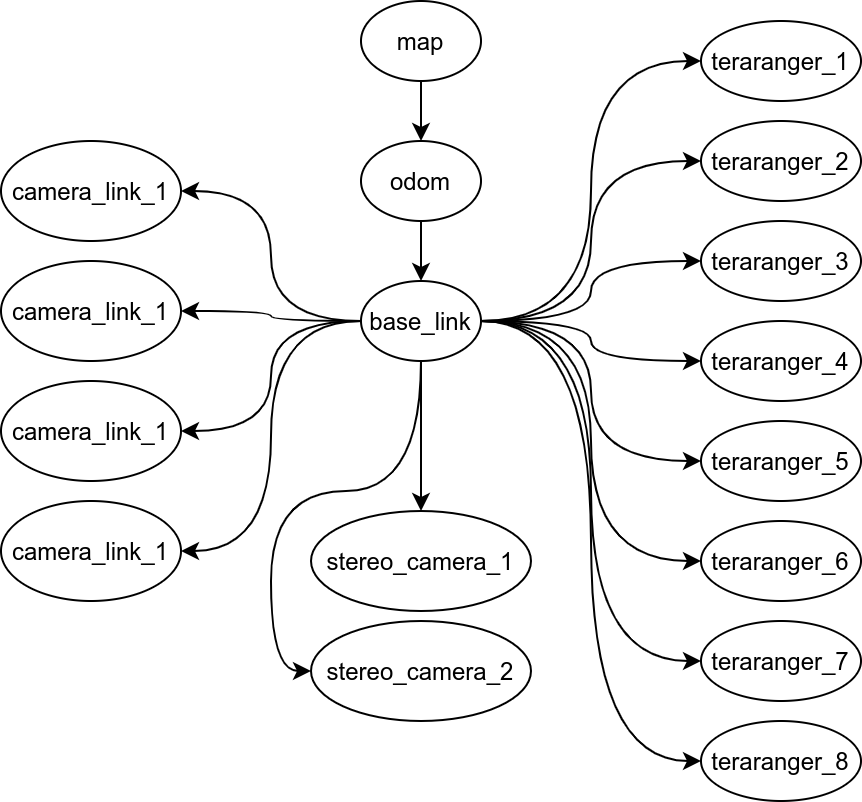
\includegraphics[width=0.5\textwidth]{Images/fig5-frames.png}
    \caption{Main reference frames in the system.}
    \label{fig:chapter2:drone:frames:frames}
\end{figure}

Finally, there is a transformation that worth mentioning: the \ac{NED} to \ac{ENU}. As mentioned in Section~\ref{sec:chapter1:ros}, ROS uses the ENU convention, while the convention adopted by the Aerospace community is the NED. Also, as mentioned in Section~\ref{sssec:chapter2:drone:mavlink}, MAVROS is in charge of doing and publish this transformation. In Figure~\ref{fig:chapter2:drone:frames:enu2ned} a simple scheme of the transformation can be seen. As explained before, this transform consists on rotating the X-axis and the Y-axis by 90 degrees, hence the homogeneous rotation matrix will have the following form:
\begin{align}
    R_{ENU}^{NED} & = \begin{bmatrix}
        0 & -1 & 0 & 0 \\
        0 & 0 & 1 & 0 \\
        -1 & 0 & 0 & 0 \\
        0 & 0 & 0 & 1
    \end{bmatrix}
\end{align}


\begin{figure}
    \centering
    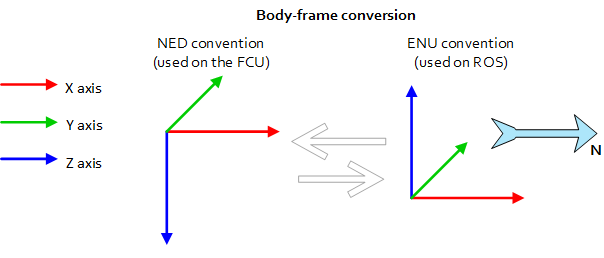
\includegraphics[width=\textwidth]{Images/fig6-ned2enu.png}
    \caption{NED to ENU conversion scheme. \cite{mavros}}
    \label{fig:chapter2:drone:frames:enu2ned}
\end{figure}

\section{Motion Model}
\label{sec:chapter2:prediction}
During the prediction step, the motion model and the covariance matrix update are computed. The motion model will update the state vector, which will store the position X, Y and Z in the global reference frame, and the orientation in the Z-axis of the drone. Fortunately MAVROS provides a node that makes odometry estimation based on different sensors outputs. The messages published by the odometry node, of type \inlinesrc{Odometry}, provide the linear velocity, the angular velocity and pose information. The velocity information is used to estimate the position in X, Y and Z, and the drone's orientation along the Z-axis. However, the velocity estimation provided by MAVROS is relative to the body reference frame, and this has to be transformed into the world reference frame, so before estimating the global position of the drone it is mandatory to do this transformation.

\begin{align}
    u &= \begin{bmatrix} v_x^b & v_y^b & v_z^b & \omega_x^b & \omega_y^b & \omega_z^b & \phi^b & \theta^b & \psi^b \end{bmatrix}^T\\
    v^w &= \textbf{T} * \begin{bmatrix} v_x^b \\ v_y^b \\ v_z^b \end{bmatrix}
\end{align}
where the control vector $u$ is composed by the linear velocities in the body reference frame ($v_x^b$, $v_y^b$, $v_z^b$), the angular velocities in the body reference frame ($\omega_x^b$, $\omega_y^b$, $\omega_z^b$) and the drone's orientation ($\phi^b$, $\theta^b$, $\psi^b$). Additionally, $\textbf{T}$ is the homogeneous transform (see Section~\ref{sec:chapter1:transform}) using the current orientation of the drone: $\phi^b$, $\theta^b$ and $\mu_{\psi}$. Notice the third element of the orientation ($\mu_{\psi}$), this is because the orientation over the Z-axis is estimated by the filter. As result, $v^w$ will be a column vector with the linear velocities in the global reference frame. \\

Given this, the motion model update can be summarized in the following calculation:
\begin{align}
    \hat\mu &=
    \begin{bmatrix}
        \mu_{t-1, x^w} \\ \mu_{t-1, y^w} \\ \mu_{t-1, z^w}
    \end{bmatrix}
    + \Delta t * v^w \\
    \hat\mu_{\psi} &= \mu_{t-1, \psi} + \Delta t * \omega_z^b
\end{align}

Then, $\textbf{G}_t$, which is the Jacobian matrix of the motion model, should be computed. As mentioned in Section~\ref{subsec:chapter1:slam:ekfslam}, it has the following characteristic:
\begin{align}
    G_t &= \begin{bmatrix}
        G_r & \textbf{0} \\
        \textbf{0} & \textbf{I}
    \end{bmatrix}\\
    G_r &= \begin{bmatrix}
        1 & 0 & 0 & G_{r, 14} \\
        0 & 1 & 0 & G_{r, 24} \\
        0 & 0 & 1 & 0 \\
        0 & 0 & 0 & 1
    \end{bmatrix}
\end{align}
\begin{align*}
     G_{r, 14} &= -\Delta t * (v_y^w * (c_{\phi} * c_{\psi} + s_{\theta} * s_{\phi} * s_{\psi}) - v_z^w * (c_{\psi} * s_{\phi} - c_{\phi} * s_{\theta} * s_{\psi}) + v_x^w * c_{\theta} * s_{\psi}) \\
     G_{r, 24} &= -\Delta t * (v_z^w * (c_{\psi} * s_{\phi} + c_{\phi} * s_{\theta} * c_{\psi}) -v_y^w * (c_{\phi} * s_{\psi} - s_{\theta} * s_{\phi} * c_{\psi}) + v_x^w * c_{\theta} * s_{\psi})
\end{align*}
where
\begin{alignat*}{3}
    c_{\phi} &= \cos{\left(u_{\phi}\right)}, \quad & c_{\theta} &= \cos{\left(u_{\theta}\right)}, \quad & c_{\psi} &= \cos{\left(\mu_{\psi}\right)} \\
    s_{\phi} &= \sin{\left(u_{\phi}\right)}, \quad & s_{\theta} &= \sin{\left(u_{\theta}\right)}, \quad & s_{\psi} &= \sin{\left(\mu_{\psi}\right)}
\end{alignat*}\\
The function $g$ that models the motion of the drone is assumed to be perfect and therefore noise free. So, before computing the covariance update, it is necessary to compute the process noise covariance matrix ($R_t$) that encodes the motion model noise which, in this case, is related to the underlying dynamics of the drone flight. The noise is assumed to be additive and Gaussian, and therefore, the motion model can be decomposed as:
\begin{equation}
    x_t = g(u_t, x_{t-1}) + \mathcal{N}\left(0, R_t\right)
    \label{eq:chapter2:prediction:motion_w_noise}
\end{equation}
\begin{equation}
    R_t = N * U * N^t
    \label{eq:chapter2:prediction:control_cov}
\end{equation}
the noise part in equation (\ref{eq:chapter2:prediction:motion_w_noise}) relates to the acceleration component that is, in this case, unknown. However, it is known from a theoretical perspective: the acceleration component in an accelerated movement is $\frac{1}{2}\Delta t^2 a$, where $a$ is the body's acceleration. Given this, we can assume that the noise component in the motion model is:
\begin{equation}
    \mathcal{N}\left(0, R_t\right) = \frac{1}{2} \Delta t^2 T_w^b \begin{bmatrix}
        a_x \\ a_y \\ a_z \\ a_{\psi}
    \end{bmatrix}
\end{equation}
where $T_w^b$ is the transformation matrix from body to world reference frame. The covariance of the process noise ($R_t$) can be decompose as shown in equation~(\ref{eq:chapter2:prediction:control_cov}), where matrix $N$ is the Jacobian of acceleration term  with respect to the state vector, and matrix $U$ is the estimated average acceleration.
\begin{equation}
    N = \frac{\partial \frac{1}{2} \Delta t^2 T_w^b \textbf{a}}{\partial \mu}
\end{equation}
\begin{equation}
    U = \textbf{I} * \begin{bmatrix}
        a_{avg, x} \\ a_{avg, y} \\ a_{avg, z} \\ a_{avg, \psi}
    \end{bmatrix}
\end{equation}
The multiplication in (\ref{eq:chapter2:prediction:control_cov}) provides an approximate mapping between the motion noise in control space and the motion noise in the state space.\\

Finally, the covariance update should be computed as follow
\begin{align}
    \hat\Sigma &= G_t * \Sigma * G_t^T + R_t
\end{align}

\section{Observation Models}
\label{sec:chapter2:correction}
While the drone is moving around the environment it senses different landmarks that may be included or not in the state vector. These observations will eventually improve the localization of the drone, and will improve the landmarks' poses if needed. The whole process involves the computation of the Jacobian of the observation model for the seen landmark, the computation of the Kalman gain, and the update of the state vector and covariance matrix.\\

To perform the correction step, EKF-SLAM needs a linearized observation model with additive Gaussian noise. In the case studied in this work, there are two kinds of landmarks and, therefore, two different observation models. The main difference between these two type of landmarks, is that the position of poles type is known, while it is not known in the case of markers. Hence, every time the robot "sees" a pole, the algorithm will update the drone's pose and the known markers' pose; while every time it "sees" a marker two course of action are possible:
\begin{enumerate}[a)]
    \item{if the marker is not known, it is added to the state vector, enlarging it along with the covariance matrix.}
    \item{if the marker is known, its pose, the pose of all other markers, and the drone's pose are updated.}
\end{enumerate}

The observation model is, as with the motion model in equation~(\ref{eq:chapter2:prediction:motion_w_noise}), assumed to be perfect and with an additive Gaussian noise. The noise here is related to the observation process, and so, related to the used sensors.
\begin{equation}
    z_i = h_i\left(x_t\right) + \mathcal{N}\left(0, Q_t\right)
    \label{eq:chapter2:correction:obs_w_noise}
\end{equation}
Consequently, the noise covariance matrix of the observation model cannot be deducted as with the noise covariance matrix of the motion model. In this case, the matrix should be constructed empirically based on the sensors' characteristics, and it has the following characteristic:
\begin{equation}
    Q_t = \begin{bmatrix}
        \sigma_1^2 &  & \textbf{0} \\
         & \ddots & \\
        \textbf{0} & & \sigma_n^2 \\
    \end{bmatrix}
\end{equation}\\
where the diagonal elements $\sigma_{1..n}$ are the standard deviation of the sensor. Depending on the sensor used, the diagonal elements can be the standard deviation for the range and bearing components (distance, azimuth and elevation), or others.\\

As shown in Algorithm~\ref{alg:chapter1:slam:ekfslam} several steps are followed during the correction part of the algorithm. After computing the observation model and its Jacobian matrix, the Kalman gain and the innovation should be calculated, and finally, the state vector and covariance matrix updates should be done.

\subsection{Observation model for Poles}
\label{subsec:chapter2:correction:poles}
In the case of Poles, a range and bearing method is used. In this case, since the poles have a known position, their information is not kept in the state vector and therefore, this information will be used for localization purposes.\\

A ROS node will publish the range and bearing information every time the drone sees a pole, and this information will be used to calculate the innovation based on the predicted range and bearing. Hence, the observation model used for poles is computed in the following way:
\begin{equation}
    \begin{bmatrix}
        p_{i, x}^b \\ p_{i, y}^b \\ p_{i, z}^b
    \end{bmatrix} = \bm{T_r}^{-1} \begin{bmatrix}
        p_{i, x}^w \\ p_{i, y}^w \\ p_{i, z}^w
\end{bmatrix}
\label{eq:chapter2:correction:pole:world2body_transform}
\end{equation}
\begin{equation}
    h_i(\hat\mu_t) = \begin{bmatrix}
        p_{i, \rho} \\ p_{i, \alpha} \\ p_{i, \beta}
    \end{bmatrix} = \begin{bmatrix}
    \sqrt{ p_{j, x^b}^2 + p_{j, y^b}^2 } \\
    \atantwo{p_{j, y}^b}{p_{j, x}^b} \\
    \atantwo{p_{j, z}^b}{p_{j,\rho}^b}
\end{bmatrix}
\label{eq:chapter2:correction:pole:range_bearing}
\end{equation}

In equation~(\ref{eq:chapter2:correction:pole:world2body_transform}), $\bm{T_r}^{-1}$ corresponds to the inverse of the homogeneous transformation matrix with respect to the current drone's pose, and elements $p_i^w$ are the $x$, $y$ and $z$ coordinates of the $i$ pole's tip in the world reference frame. This way, the global position of the pole $i$ is projected to the body reference frame. After that, the range ($\rho$), azimuth angle ($\alpha$) and elevation angle ($\beta$) are calculated, as shown in equation~(\ref{eq:chapter2:correction:pole:range_bearing}). In Figure~\ref{fig:chapter2:correction:poles:range_bearing} an example of the range and bearing is shown.
\begin{figure}[h]
    \centering
    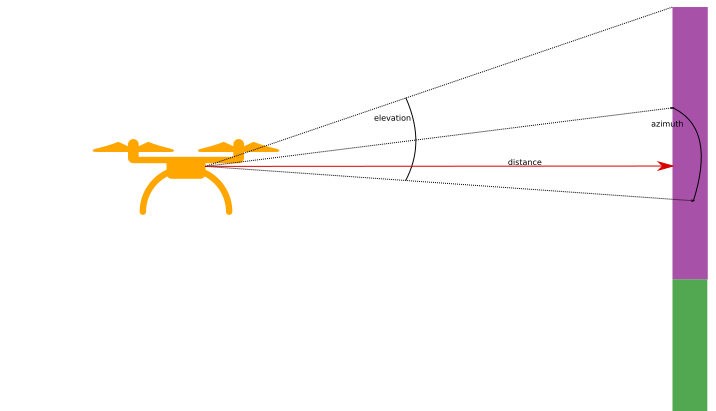
\includegraphics[width=\textwidth]{Images/fig7-range_and_bearing}
    \caption[Range and Bearing example]{Range and bearing example. The drone observes a pole, process the data from the sensors and estimates the distance ($\rho$), the elevation angle ($\beta$), and the azimuth angle ($\alpha$). The elevation angle is calculated based on the top extreme of the pole.}
    \label{fig:chapter2:correction:poles:range_bearing}
\end{figure}

Observing a pole affects only the drone's pose, and therefore, the Jacobian matrix of the observation model will have the following form:
\begin{equation}
    H_i = \begin{bmatrix}
        \frac{\partial \rho'}{\partial \mu_x} & \frac{\partial \rho'}{\partial \mu_y} & \frac{\partial \rho'}{\partial \mu_z} & \frac{\partial \rho'}{\partial \mu_{\psi}} & \dots & 0 \\
        \frac{\partial \alpha'}{\partial \mu_x} & \frac{\partial \alpha'}{\partial \mu_y} & \frac{\partial \alpha'}{\partial \mu_z} & \frac{\partial \alpha'}{\partial \mu_{\psi}} & \dots & 0 \\
        \frac{\partial \beta'}{\partial \mu_x} & \frac{\partial \beta'}{\partial \mu_y} & \frac{\partial \beta'}{\partial \mu_z} & \frac{\partial \beta'}{\partial \mu_{\psi}} & \dots & 0
    \end{bmatrix}
\end{equation}
where $\rho'$ corresponds to the distance part of the observation model, $\alpha'$ is the azimuth part, and $ \beta'$ the elevation part. The elements after the \nth{4} column are all 0, which means, as said before, that the observation of a pole will not affect the pose of the markers.

\subsection{Observation model for Markers}
\label{subsec:chapter2:correction:markers}

The observation model for the markers is a bit different. In this case a ROS node is responsible of detecting, tracking and publishing the pose of the markers with respect to the camera that has seen it. The ROS package responsible of this process is called \inlinesrc{visp_auto_tracker}, and publishes messages of type \inlinesrc{PoseStamped}, which provides the position and orientation of the seen marker. An example of this situation can be seen in Figure~\ref{fig:chapter2:correction:markers:example}.\\

\begin{figure}
    \centering
    \includegraphics[width=\textwidth]{Images/fig8-marker_example}
    \caption[Example of the drone observing a marker]{Example of the drone observing a marker. The camera visualize a marker and the node \inlinesrc{visp_auto_tracker} estimates its pose with respect to the camera reference frame.}
    \label{fig:chapter2:correction:markers:example}
\end{figure}

Every time the camera that points down sees a known marker, the \inlinesrc{visp_auto_tracker} node will publish the pose of that marker. This published pose is with respect to the camera which is not positioned at the drone's center of mass and so, a different transformation is needed. This process can be seen in equation~(\ref{eq:chapter2:correction:markers:world2body_trasnform}), in which the transformation of the marker's pose in the world reference frame is transformed to the pose in the camera reference frame.
\begin{equation}
    \begin{bmatrix}
        m_{i, x}^c \\ m_{i, y}^c \\ m_{i, z}^c \\ m_{i, \phi}^c \\ m_{i, \theta}^c \\ m_{i, \psi}^c
    \end{bmatrix} = (\bm{T_r} * \bm{T_c})^{-1} * \bm{T_m}
    \label{eq:chapter2:correction:markers:world2body_trasnform}
\end{equation}
where, $\bm{T_r}$ is the homogeneous transformation matrix of the drone's pose, $\bm{T_c}$ is the homogeneous transformation matrix of the camera's pose, and $\bm{T_m}$ is the homogeneous transformation of the marker's pose. The result is a vector that contains the marker's pose in the camera reference frame.\\

As mentioned before, observing a marker will update the drone's pose and that marker's pose, and therefore the Jacobian matrix of the observation model will have a different aspect from the pole's case. Here, the Jacobian can be split in two parts as shown in equation~(\ref{eq:chater2:correction:markers:jacobian}), where the left part, as with the poles, affects the drone's pose, while the right part of the matrix affects the seen marker's pose.
\begin{align}
    H_i &= \begin{bmatrix}
        \frac{\partial h_i(\hat\mu)}{\partial \mu_r} & \dots0\dots & \frac{\partial h_i(\hat\mu)}{\partial \mu_{m_i}} & \dots0\dots
    \end{bmatrix}
    \label{eq:chater2:correction:markers:jacobian}
\end{align}

The Jacobian matrices of the observation model with respect to the drone state and with respect the marker pose can be seen in Appendix~\ref{appendix:a}. It is worth to mention that the reason why this matrix only contains two sections different to zero is because of the relations between markers: observing a marker does not affect the pose of others, and therefore, the Jacobians of the observation model for marker $i$ with respect to marker $i+1$ or any other marker is 0.\\

Furthermore, unlike the case of poles, the markers' pose is unknown the first time, and therefore the algorithm will introduce their pose into the state vector when the drone sees a previously unknown marker.

\subsubsection{Adding new Markers}
\label{subsubsec:chapter2:correction:markers:add}
\nocite{slam-auto-mob-robots}
As mentioned in Section~\ref{subsec:chapter1:slam:ekfslam:addlandmarks}, to add new landmarks to the state vector an inverse observation model is needed. In the current case, the inverse observation model will project the observed marker's pose from the camera reference frame to the world reference frame. Equation~\ref{eq:chapter2:correction:markers:inverseh} shows the inverse observation model for markers where, similarly to the observation model, a set of transformations are performed but, this time, in order to obtain the pose of the seen marker in the world reference frame:
\begin{align}
    \begin{bmatrix}
        m_{i, x}^w \\ m_{i, y}^w \\ m_{i, z}^w \\ m_{i, \phi}^w \\ m_{i, \theta}^w \\ m_{i, \psi}^w
    \end{bmatrix} &= \bm{T_r} * \bm{T_c} * \bm{T_m}
    \label{eq:chapter2:correction:markers:inverseh}
\end{align}

As before, $\bm{T_r}$ is the homogeneous transformation matrix of the drone's pose, $\bm{T_c}$ is the homogeneous transformation matrix of the camera's pose, and $\bm{T_m}$ is the homogeneous transformation of the marker's pose. The result is a vector containing the marker's pose in the world reference frame, and with which will extend the state vector:
\begin{align*}
    \mu_t = \left[\begin{array}{c|cccccc}
        \mu_t & m_{i, x}^w & m_{i, y}^w & m_{i, z}^w & m_{i, \phi}^w & m_{i, \theta}^w & m_{i, \psi}^w
    \end{array}
    \right]^T
\end{align*}

Furthermore, the covariance matrix should be updated in order to contain the newly added marker. As shown in equation~\ref{eq:chapter1:slam:ekfslam:cov_update}, the Jacobian of the inverse observation model with respect to the drone's state and the Jacobian of the inverse observation model with respect to the marker's state are needed. Both Jacobian matrices can be seen in Appendix~\ref{appendix:a}. In this case, the matrix $\bm{Y_x}$ has a size of ($\norm{\mu}+6) \times (\norm{\mu})$ where $\norm{\mu}$ is the size of the state vector before adding the projected pose of the seen marker. On the other hand, the matrix $\bm{Y_z}$ has a size of $(\norm{\mu}+6) \times 6$. Given these two matrices, the new covariance matrix $\Sigma$ will be increased by 6 columns and 6 rows and will have the following form:
\begin{align*}
    \Sigma = \begin{bmatrix}
        \Sigma_{r,r} & \Sigma_{r,m} \\ \Sigma_{r,m} & \Sigma_{m,m}
    \end{bmatrix}
\end{align*}
where $\Sigma_{r,r}$ is the covariance matrix between the drone's state variables, the $\Sigma_{r,m}$ and $\Sigma_{m,r}$ is the covariance matrix between the drone and the markers' state variables, and between the markers and the drone's state variables, and $\Sigma_{m,m}$ is the covariance matrix between markers' state variables.

\section{Overall Architecture}
\label{sec:chapter2:arch}
The system is composed by several ROS nodes that specialize and perform a wide range of operations. However, what is most interesting for this work is the node that is in charge of the EKF-SLAM process. \\

In Figure~\ref{fig:chapter2:architecture:components} the components that interact around the EKF Localization node can be seen. In the center of the figure the \inlinesrc{EKFSLAM} component is placed, which is responsible of running the EKF-SLAM algorithm. Every time an \inlinesrc{Odometry} message arrives, the prediction step takes place, and this happens every 30Hz. Furthermore, every time a \inlinesrc{RangeAndBearingPoles} or a \inlinesrc{QRCodeStamped} arrives the correction step takes place, and differently to the prediction step, this depends on whether the drone observes or not a pole or a marker. Additionally, the \inlinesrc{EKFSLAM} component provides three services:
\begin{enumerate}
    \item \inlinesrc{get_drone_state}: takes no arguments, and returns the current localization of the drone \inlinesrc{Pose} message.
    \item \inlinesrc{get_marker_state}: takes as argument the id of a marker, and returns the current estimated pose of that marker\inlinesrc{Pose} message.
    \item \inlinesrc{save_map}: takes no arguments, and it saves the current map in a YAML file. The map contains the pose of all the poles and all the markers seen so far.
\end{enumerate}

\begin{figure}
    \centering
    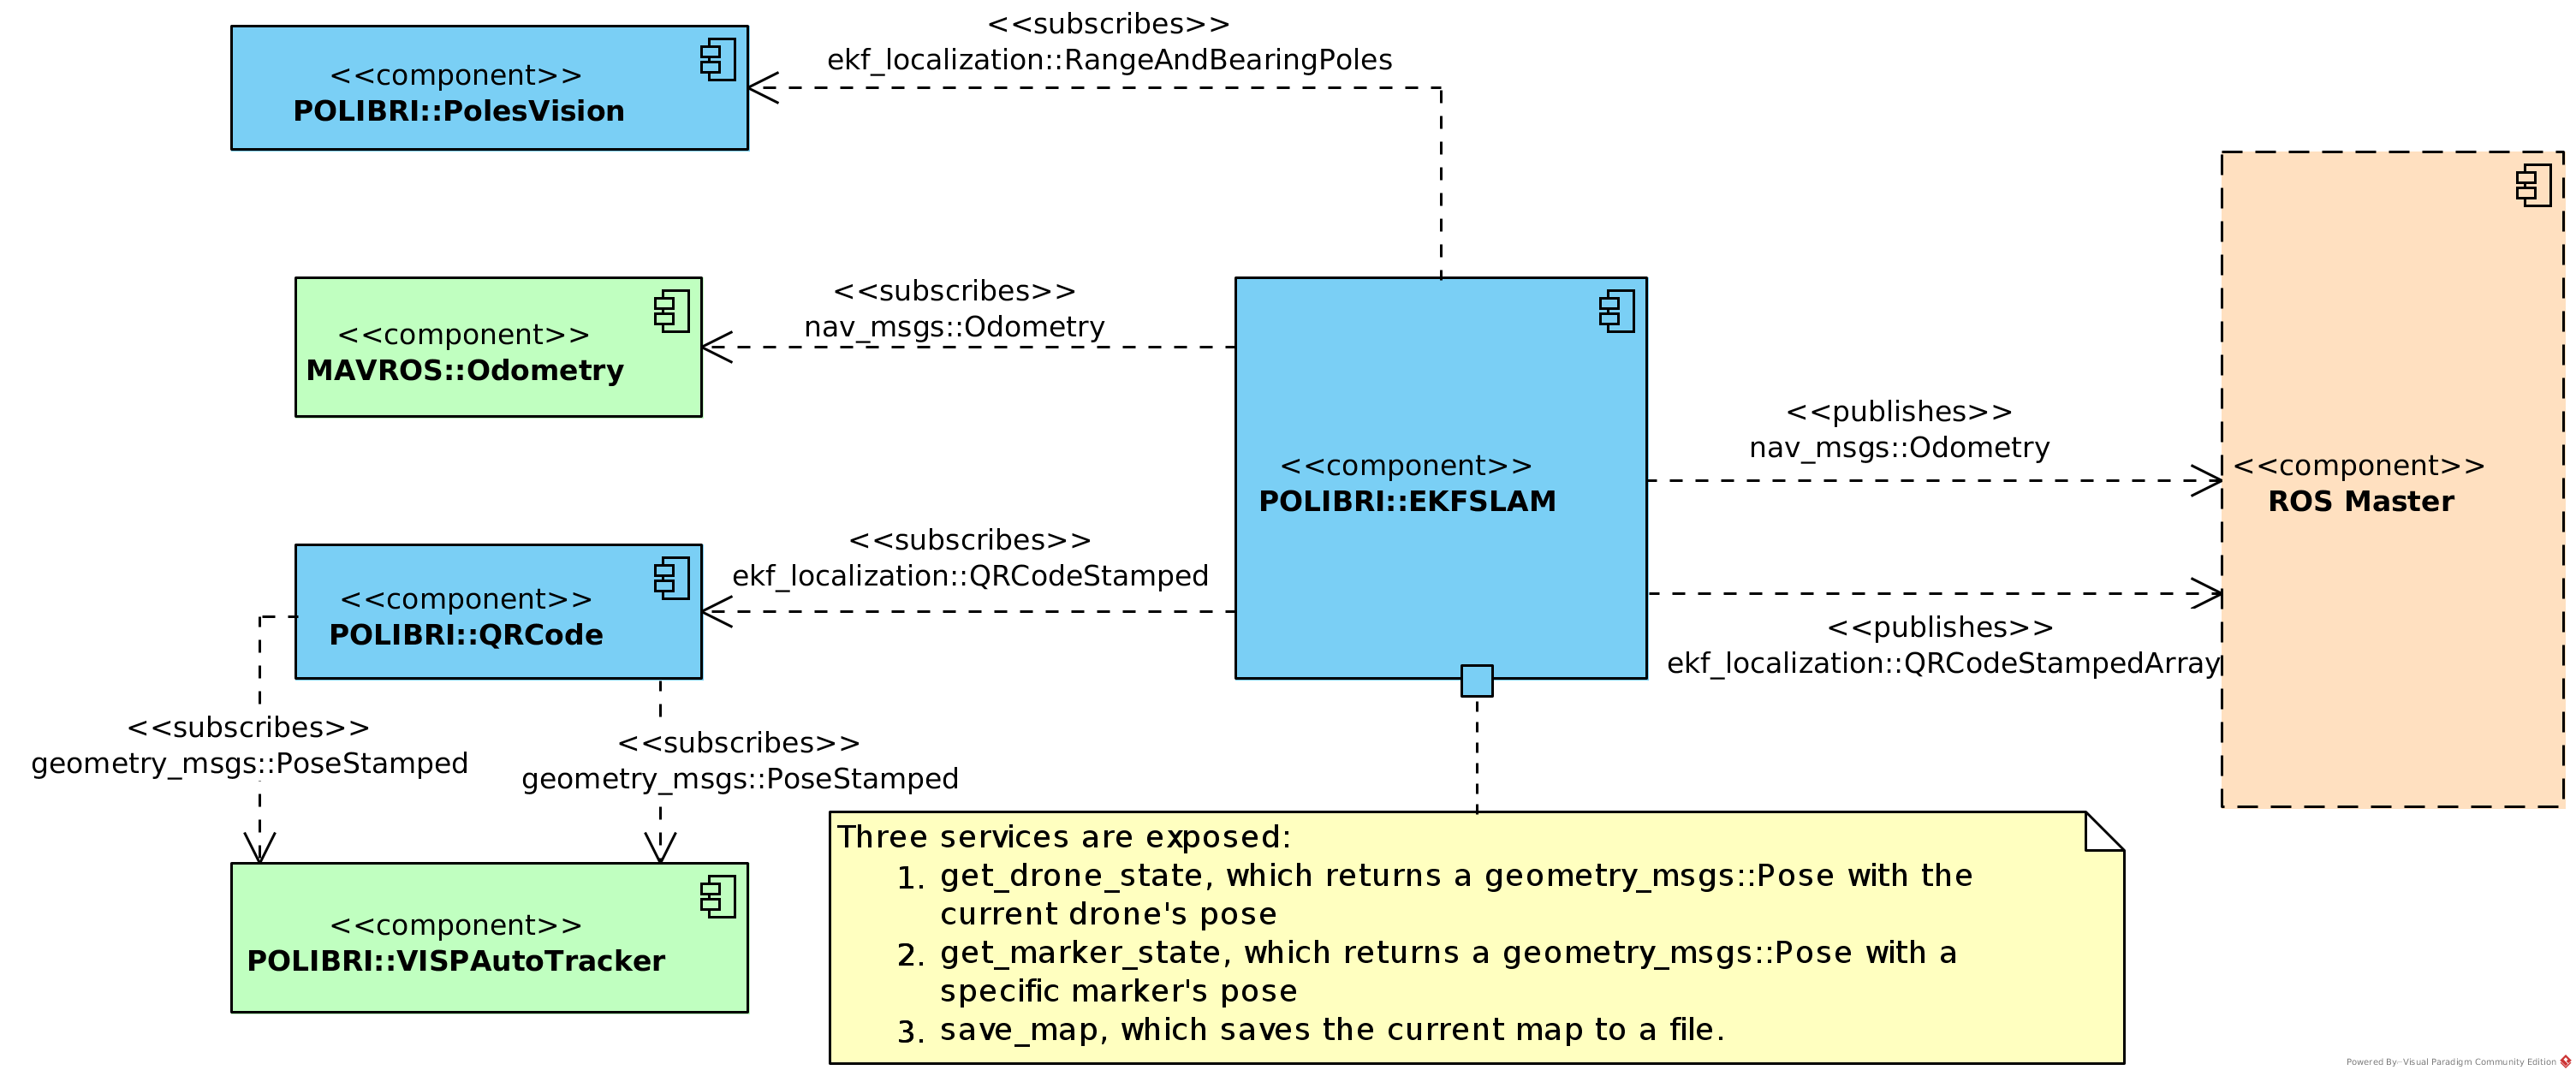
\includegraphics[width=\textwidth]{Images/fig9-components_diagram}
    \caption[Components diagram of the EKF Localization node]{Components diagram of the EKF Localization node. The \inlinesrc{EKFSLAM} class subscribes to different messages, between them the \inlinesrc{Odometry} messages are used as control variables, while the \inlinesrc{RangeAndBearingPole} and \inlinesrc{QRCodeStamped} messages are used every time the drone observes a pole or a marker. Moreover, \inlinesrc{EKFSLAM} class publishes two types of messages: \inlinesrc{Odometry} which provides the filtered localization and \inlinesrc{QRCodeStampedArray} which contains a list markers' poses.}
    \label{fig:chapter2:architecture:components}
\end{figure}

It is worth to mention that the messages of type \inlinesrc{QRCodeStamped} are provided by the \inlinesrc{QRCode} node which is internal to the \inlinesrc{ekf_localization} package. This node is needed because the \inlinesrc{visp_auto_tracker}, responsible of identifying the markers and publish their poses, publish these data as separate messages: the marker's id as a \inlinesrc{String} message and the pose as a \inlinesrc{PoseStamped} message. Due to this situation, the \inlinesrc{QRCode} node is responsible of match both data together and publish an \inlinesrc{QRCodeStamped} message which contains the marker's identifier and its pose.\\

\begin{figure}
    \centering
    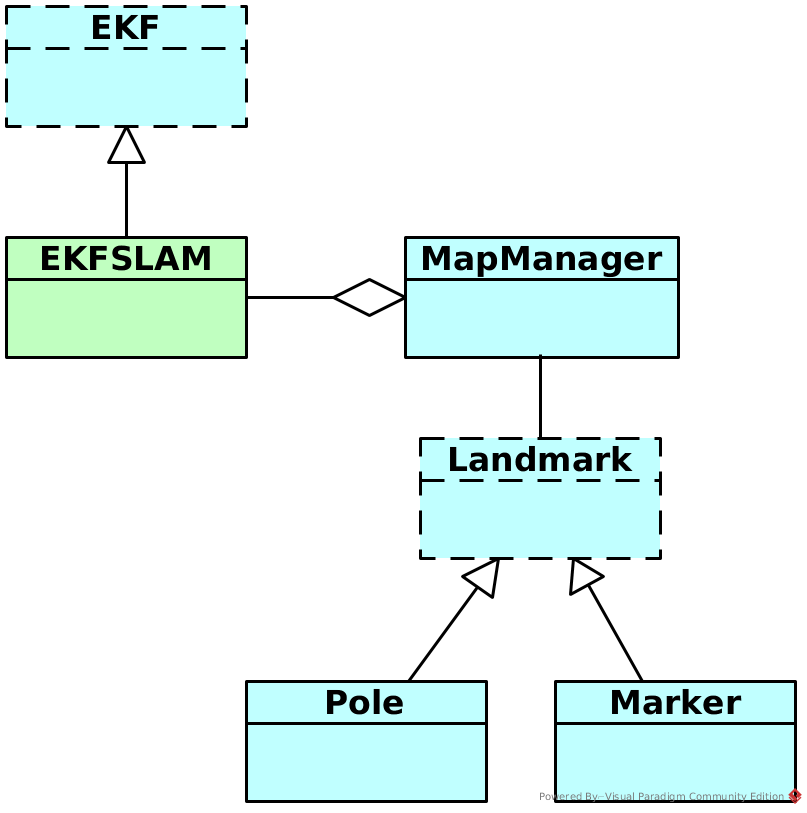
\includegraphics[width=0.5\textwidth]{Images/fig10-class_diagram}
    \caption[Class diagram of the EKFSLAM node]{Class diagram of the EKFSLAM node. The \inlinesrc{EKFSLAM} class is composed by a \inlinesrc{MapManager} instance, which is composed by a list of \inlinesrc{Landmarks}. The \inlinesrc{Landmark} class is abstract and its concrete classes are \inlinesrc{Pole} and \inlinesrc{Marker}.}
    \label{fig:chapter2:architecture:class}
\end{figure}

The main element of the EKF-SLAM node is the \inlinesrc{EKFSLAM} class which is responsible of keeping track of the state vector and execute the EKF-SLAM algorithm. This class inherit from an abstract class called \inlinesrc{EKF}, which is responsible of the implementation of the algorithm in a generic way, while the specifics for the current problem is contained in its child.\\

There are several components that interact within \inlinesrc{EKFSLAM} class, but probably the most interesting one is the \inlinesrc{MapManager} class. This class is responsible of maintaining an updated map of the environment with all the poles and markers, and to save and retrieve the map from a YAML file.\\

The \inlinesrc{MapManager} class contains a list of \inlinesrc{Landmark}s, and every time the state vector is updated in \inlinesrc{EKFSLAM} class, the \inlinesrc{MapManager} class updates the information about each \inlinesrc{Marker}. As mentioned before, the pose of each pole is known and needs no update. Furthermore, the \inlinesrc{Landmark} class is specialized in a \inlinesrc{Marker} class and a \inlinesrc{Pole} class, each of which is responsible of provide the observation model associated to it and the needed Jacobian matrices for the algorithm, hiding the implementation to the \inlinesrc{EKFSLAM} class.
\subsection{ROS nodes}
\label{subsec:chapter2:arch:nodes}
Regarding the ROS node that comprise the system, in Figure~\ref{fig:chapter2:architecture:nodes:all} all the ones that interact with the localization node are shown. The EKF-SLAM node is called \inlinesrc{/ekf_localization_node}, and as mentioned before, it interacts with \inlinesrc{/mavros} node, all the poles identification nodes (\inlinesrc{/poles_vision_#}), the \inlinesrc{/qr_code_node} which publishes the markers position with its identifier, and the \inlinesrc{/rtabmap} node that provides the Octomap messages. \\

As mentioned, the Figure~\ref{fig:chapter2:architecture:nodes:all} shows all the nodes (depicted as ellipses) with its interactions: a node publishes a message topic, and the topic is consumed by a node. This interaction is represented by the arrows, where an incoming arrow means that a node subscribes to the message topic, while an outgoing arrow means that the node publishes that message topic. Arrows go from a node to a topic or from a topic to a node, but do not go from node to node. Its reason lies on the fact that nodes interact between each other using a message passing interface as mention in Section~\ref{sec:chapter1:ros}. Furthermore, it is worth to mention that in Figure~\ref{fig:chapter2:architecture:nodes:all} a \inlinesrc{/gazebo} node is present. This node appears only on simulation and represents the simulated environment, that is why it publishes all the cameras and stereo cameras information.\\
\begin{figure}
    \centering
    \includegraphics[width=\textwidth]{Images/fig11-rosgraph_all}
    \caption[ROS graph of the system]{ROS graph of the system. Nodes are depicted as ellipses, while message topics are depicted as boxes. Each arrow means that a node publishes or subscribes to a specific message topic.}
    \label{fig:chapter2:architecture:nodes:all}
\end{figure}
Figure~\ref{fig:chapter2:architecture:nodes:ekf_node} shows the detail for the \inlinesrc{/ekf_localization_node} with all its subscriptions. It is worth to mention the \inlinesrc{/qr_code_node}, which subscribes to \inlinesrc{/visp_auto_tracker/code_message} and \inlinesrc{/visp_auto_tracker/object_position}, and publishes a \inlinesrc{/visp_auto_tracker/stamped_object_position}.
\begin{figure}[h]
    \centering
    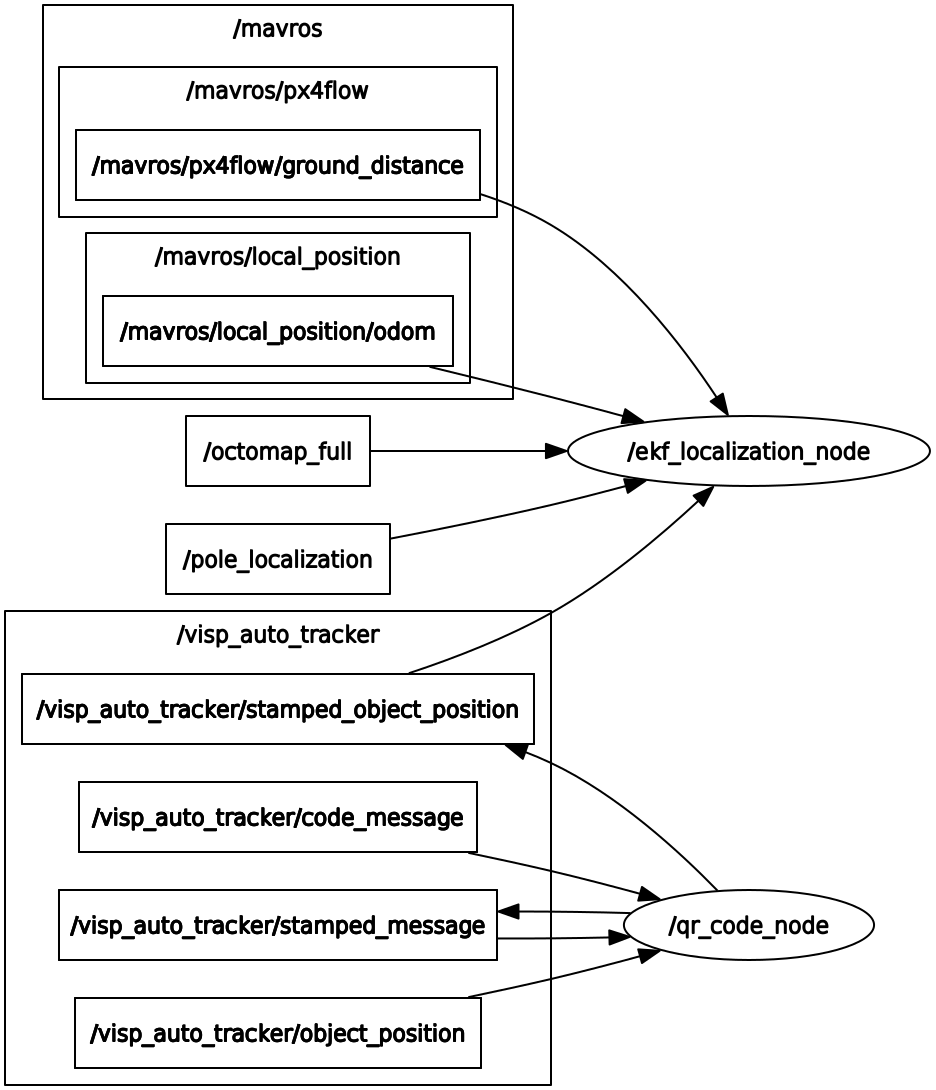
\includegraphics[width=0.8\textwidth]{Images/fig12-rosgraph_ekf_node}
    \caption[Detail of the EKF-SLAM node interactions]{Detail of the EKF-SLAM node interactions. Beside the \inlinesrc{/ekf_localization_node}, the \inlinesrc{/qr_node_code} can be seen. This node, is responsible of subscribing the \inlinesrc{/visp_auto_tracker} messages in order to, then, publish the identifier along with the pose of the marker that has been seen. On the other hand, the \inlinesrc{/ekf_localization_node} subscribes to the \inlinesrc{/mavros}, \inlinesrc{/octomap}, \inlinesrc{/pole_localization} and \inlinesrc{/visp_auto_tracker} messages.}
    \label{fig:chapter2:architecture:nodes:ekf_node}
\end{figure}




















 % Include the second content chapter
%\chapter{Experimental Results}
\label{chapter3}

% Introduction where I should explain the purpose of the experiments.

\section{The Environment}
\label{sec:chapter3:environment}

\section{Simulated Experiments}
\label{sec:chapter3:simulation}

\subsection{Procedures}
\label{subsec:chapter3:simulation:procedures}

\subsection{Results}
\label{subsec:chapter3:simulation:results}

\section{Empirical Results ?}
\label{sec:chapter3:empirical}

\subsection{Procedures}
\label{subsec:chapter3:empirical:procedures}

\subsection{Results}
\label{subsec:chapter3:empirical:results} % Include the third content chapter

\backmatter

\chapterstyle{default} % Reset the chapter style back to the default used for non-content chapters

%----------------------------------------------------------------------------------------
%	BIBLIOGRAPHY
%----------------------------------------------------------------------------------------

\bibliographystyle{plainnat} % Use the plainnat bibliography style

\bibliography{bibliography} % Use the bibliography.bib file as the source of references

%----------------------------------------------------------------------------------------
%	INDEX
%----------------------------------------------------------------------------------------

\printindex % Print the index

%----------------------------------------------------------------------------------------

\end{document}